% !TEX encoding = UTF-8 Unicode
% !TEX spellcheck = en
% spell-checker:ignore RWTH, leavevmode, qedhere, siunitx, titlehead
\documentclass[fleqn,bibliography=totoc,index=totoc,paper=A4,twoside=semi,DIV=12]{scrbook}
\usepackage[american]{babel}
\usepackage[T1]{fontenc}
\usepackage[utf8]{inputenc}
% spell-checker:disable
% Restore the typical KOMA-Script style fonts, which are changed by setting fontenc to T1
\usepackage{lmodern}
\DeclareSymbolFont{largesymbols}{OMX}{cmex}{m}{n} % use cmex rather than lmex
% spell-checker:enable
\usepackage{styleBB}
\usepackage{bm}
\usepackage{multirow}
\usepackage{algorithm2e}
\usepackage{nicefrac}
\usepackage{afterpage}
\usepackage{graphicx}
\usepackage{caption}
\usepackage{subcaption}
\usetikzlibrary{positioning}
\usepackage[symbols,nogroupskip,sort=none]{glossaries-extra}
\usepackage[utf8]{inputenc}
\usepackage{pgfplots}
\DeclareUnicodeCharacter{2212}{−}
\usepgfplotslibrary{groupplots,dateplot}
\usetikzlibrary{patterns,shapes.arrows}
\pgfplotsset{compat=newest}
% \usepackage[acronym]{glossaries}
% \usepackage{algorithm}
% \usepackage{algpseudocode}
% \usepackage{algorithmic}
% \usepackage{silence}
% \WarningFilter{latex}{Marginpar on page}

\setlength{\marginparwidth}{2cm}
\usepackage[textsize=tiny]{todonotes}

\graphicspath{
{./figures/},
}

\pgfplotsset{
  table/search path={data},
}

\addbibresource{thesis.bib}

\renewcommand{\chaptermark}[1]{\markboth{\thechapter\,\,#1}{}}
\renewcommand{\sectionmark}[1]{\markright{\thesection\,\,#1}}
\newtheorem{problem}{Problem}
% \newcommand{\vct}[1]{\bm{#1}}
\usepackage[headsepline]{scrlayer-scrpage}
\clearpairofpagestyles
\addtokomafont{pagehead}{\normalfont\bfseries}
\lohead{\rightmark}
\rohead{\thepage}
\lehead{\thepage}
\rehead{\leftmark}

\makeindex

% Useful to build the dvi/pdf without any images
%\renewcommand{\includegraphics}[2][a]{image}
% Useful to let jpg be preferred to png by \includegraphics (default behavior is the other way round) if no suffix is specified.
%\DeclareGraphicsExtensions{.pdf,.jpg,.png}





\begin{document}

% % Get rid of the double spacing at the end of a sentence.
\frenchspacing
% Configure the "depth" of the table of contents
\setcounter{tocdepth}{2}
% Change the numbering of the first enumerated list to (i)
\renewcommand{\labelenumi}{(\roman{enumi})}
% Change the numbering of the second enumerated list to (1)
\renewcommand{\labelenumii}{(\arabic{enumii})}

\titlehead{%
\raggedleft

\includegraphics[scale=0.65]{./figures/rwth_aices_cmyk-crop.pdf}\\[1ex]
\centering
The present work was submitted to the\\Aachen Institute for Advanced Study in Computational Engineering Science\\
   RWTH Aachen University\\
   Junior Professorship of Mathematical Image and Signal Processing
}\subject{Master's thesis}
\title{Deep Unfolding of Wirtinger Flow Type Schemes}
\author{Ali Darijani}
\date{\today}
\publishers{
\begin{tabular}{rl}
% 1\textsuperscript{st} supervisor:&Professor Benjamin Berkels\\
supervisor:&Professor Benjamin Berkels\\
% 2\textsuperscript{nd} supervisor:&Professor Jane Q. Public
\end{tabular}
}

% \lowertitleback{typeset using {\KOMAScript} and {\LaTeX}}
\lowertitleback{Typesetted using {\TeX}, {\AmS-\TeX}, and {\KOMAScript}\\Happy \TeX-ing!}


\frontmatter

\maketitle

\tableofcontents

\mainmatter

\chapter*{}
\addcontentsline{toc}{chapter}{Dedication}  



% \clearpage
\begin{center}
    \thispagestyle{empty}
    \vspace*{\fill}
    \large TO THE MEMORY OF THE MOHAMMAD MAHDI ELYASI\\
    A DOWN TO EARTH TRtUE PHYSICIST AND A LEGENDARY PETROLHEAD
    \vspace*{\fill}
\end{center}
% \clearpage

\endinput
\chapter*{Abstract}
\addcontentsline{toc}{chapter}{Abstract}  



\acl{SDL} \ac{ISTA} \ac{LISTA} \ac{FISTA} \ac{Ada-LISTA}

\ac{DU}/\ac{AU}
Physical measurements in settings where light, electrons, and similar existences are involved will result in a phase 
loss\cite{Shechtman2015} in the mathematical formulation. The phenomenon is called \acl*{PP}\cite{Shechtman2015} 
and the methods developed to tackle the said unpleasantness are called 
\acl*{PR}\cite{Jaganathan2015}\cite{Liu2019} methods. Due to its presence in a wide spectrum of 
applications\cite{Shechtman2015}\cite{Candes2014} ranging from X-ray crystallography, transmission electron microscopy 
to quantum mechanics, the retrieval methods are highly investigated and coveted\cite{Jaganathan2015}\cite{Liu2019}. 
One of the contemporary breakthroughs are the \ac{WF}\cite{Candes2014}\cite{Liu2019} variants which are nice and relatively easy algorithms 
with small memory footprints equipped with nice guarantees on the solutions. \ac{WF}\cite{Liu2019} variants are derived from minimizing a 
certain functional and are of iterative nature. Like most iterative approaches they are certain parameters that need to be fixed which 
greatly influence the convergence rate and stability of the algorithm. While analytical guarantees are nice to have, we aim 
to investigate if it is possible for improvements of the model by altering these parameters using \ac{DU}/\ac{AU}\cite{Monga2019} 
which is an emerging technic from the data-driven world. \ac{DU}/\ac{AU} is basically unfolding/unrolling an 
iterative algorithm finite times and putting it into a neural network to be trained. \ac{ML}\ac{DL} studies are often accompanied 
by \ac{HP} which is why we close the current work by exactly doing that.   
\endinput
\chapter*{Acknowledgements}
\addcontentsline{toc}{chapter}{Acknowledgements}


1st Order Family Members:
Fatemeh Darijani, Nabiollah Darijani, 
2nd Order Family Members:





\endinput
\glsxtrnewsymbol[description={inclusion signs}]{inclusion signs}{\ensuremath{\subset,\supset}}
\glsxtrnewsymbol[description={rational field}]{rational field}{\ensuremath{\mathbb{Q}}}
\glsxtrnewsymbol[description={least upper bound}]{least upper bound}{\ensuremath{\sup}}
\glsxtrnewsymbol[description={greatest lower bound}]{greatest lower bound}{\ensuremath{\inf}}

\glsxtrnewsymbol[description={null vector}]{null vector}{\ensuremath{\boldsymbol{0}}}
\glsxtrnewsymbol[description={inner product}]{inner product}{\ensuremath{\boldsymbol{x} \cdot \boldsymbol{y}}}
\glsxtrnewsymbol[description={norm of vector $\boldsymbol{x}$}]{norm of vector x}{\ensuremath{\left| \boldsymbol{x} \right|}}
\glsxtrnewsymbol[description={sequence}]{sequence}{\ensuremath{\{x_n\}}}
\glsxtrnewsymbol[description={union}]{union}{\ensuremath{\bigcup,\cup}}
\glsxtrnewsymbol[description={intersection}]{intersection}{\ensuremath{\bigcap,\cap}}
\glsxtrnewsymbol[description={segment}]{segment}{\ensuremath{\left(a,b\right)}}
\glsxtrnewsymbol[description={interval}]{interval}{\ensuremath{\left[a,b\right]}}
\glsxtrnewsymbol[description={complement of $E$}]{complement of E}{\ensuremath{E^\mathsf{c}}}
\glsxtrnewsymbol[description={limit points of $E$}]{limit points of E}{\ensuremath{E^{'}}}
\glsxtrnewsymbol[description={closure of $E$}]{closure of E}{\ensuremath{\overline{E}}}
\glsxtrnewsymbol[description={limit}]{limit}{\ensuremath{\lim}}
\glsxtrnewsymbol[description={converges to}]{converges to}{\ensuremath{\to}}
\glsxtrnewsymbol[description={lim sup}]{lim sup}{\ensuremath{\lim \sup}}
\glsxtrnewsymbol[description={lim inf}]{lim inf}{\ensuremath{\lim \inf}}
\glsxtrnewsymbol[description={composition}]{composition}{\ensuremath{g \circ f}}
\glsxtrnewsymbol[description={right-hand limit}]{right-hand limit}{\ensuremath{f(x+)}}
\glsxtrnewsymbol[description={left-hand limit}]{left-hand limit}{\ensuremath{f(x-)}}
\glsxtrnewsymbol[description={derivatives}]{derivatives}{\ensuremath{f^{\prime}, \boldsymbol{f}(\boldsymbol{x})^{\prime}}}
\glsxtrnewsymbol[description={Riemann sums}]{Riemann sums}{\ensuremath{U(\boldsymbol{P},f),U(\boldsymbol{P},f,\alpha),L(\boldsymbol{P},f),L(\boldsymbol{P},f,\alpha)}}
\glsxtrnewsymbol[description={classes of Riemann (Stieltjes) integrable functionas}]{classes of Riemann (Stieltjes) integrable functionas}{\ensuremath{\mathcal{R},\mathcal{R}(\alpha)}}
\glsxtrnewsymbol[description={space of continiuous functions}]{space of continiuous functions}{\ensuremath{\mathcal{C}(X)}}
\glsxtrnewsymbol[description={norm}]{norm}{\ensuremath{\left|\left|\;\;\right|\right|}}
\glsxtrnewsymbol[description={exponential function}]{exponential function}{\ensuremath{\exp}}
\glsxtrnewsymbol[description={Dirichlet kernel}]{Dirichlet kernel}{\ensuremath{D_N}}
\glsxtrnewsymbol[description={gamma function}]{gamma function}{\ensuremath{\Gamma(x)}}

\glsxtrnewsymbol[description={spaces of linear transformation}]{spaces of linear transformation}{\ensuremath{L(X),L(X,Y)}}
\glsxtrnewsymbol[description={matrix}]{matrix}{\ensuremath{\left[\boldsymbol{A}\right]}}
\glsxtrnewsymbol[description={partial derivative}]{partial derivative}{\ensuremath{D_Jf}}
\glsxtrnewsymbol[description={gradient}]{gradient}{\ensuremath{\nabla f}}
\glsxtrnewsymbol[description={classes of differentiable functions}]{classes of differentiable functions}{\ensuremath{\mathcal{C}^\prime,\mathcal{C}^{\prime\prime}}}
\glsxtrnewsymbol[description={determinant}]{determinant}{\ensuremath{\det \left[\boldsymbol{A}\right]}}
\glsxtrnewsymbol[description={Jacobian}]{Jacobian_implicit}{\ensuremath{\boldsymbol{J}_f(\boldsymbol{x})}}
\glsxtrnewsymbol[description={Jacobian}]{Jacobian_explicit}{\ensuremath{\frac{\partial(y_1,\cdots,y_n)}{\partial(x_1,\cdots,x_n)}}}
\glsxtrnewsymbol[description={$k$-cell}]{k-cell}{\ensuremath{\mathbb{I}^k}}
\glsxtrnewsymbol[description={$k$-simplex}]{k-simplex}{\ensuremath{\mathbb{Q}^k}}
\glsxtrnewsymbol[description={basic $k$-form}]{basic k-form}{\ensuremath{d\boldsymbol{x}_{\boldsymbol{I}}}}
\glsxtrnewsymbol[description={multiplication symbol}]{multiplication symbol}{\ensuremath{^\wedge}}

\glsxtrnewsymbol[description={transform of $\omega$}]{transform of omega}{\ensuremath{\omega_{\boldsymbol{T}}}}
\glsxtrnewsymbol[description={boundary operator}]{boundary operator}{\ensuremath{\partial}}
\glsxtrnewsymbol[description={curl}]{curl}{\ensuremath{\nabla \times \boldsymbol{F}}}
\glsxtrnewsymbol[description={divergence}]{divergence}{\ensuremath{\nabla\cdot\boldsymbol{F}}}
\glsxtrnewsymbol[description={ring of elementary sets}]{ring of elementary sets}{\ensuremath{\mathcal{E}}}
\glsxtrnewsymbol[description={Lebesgue measure}]{Lebesgue measure}{\ensuremath{m}}
\glsxtrnewsymbol[description={measure}]{measure}{\ensuremath{\mu}}
\glsxtrnewsymbol[description={families of measurable sets}]{families of measurable sets}{\ensuremath{\mathcal{M}_F,\mathcal{M}}}
\glsxtrnewsymbol[description={positive(negative) part of $f$}]{posotove(negative) part of $f$}{\ensuremath{f^+,f^-}}
\glsxtrnewsymbol[description={characteristic function}]{characteristic function}{\ensuremath{K_{E}}}
\glsxtrnewsymbol[description={classes of Lebesgue-integrable functions}]{classes of Lebesgue-integrable functions}{\ensuremath{\mathcal{L},\mathcal{L}(\mu),\mathcal{L}^2,\mathcal{L}^2(\mu)}}


%%%%%%%%%%%%%%%%%%%%%%%%%%%%%%%%%%%%%%%%%%%%%%%%%%%%%%%%%%%%%%%%%%%%%%%%%%%%%%%%%%%%%%%%%%%%%%%%%%%%%%%%%%%%%%%%%%%%%%%
%%%%%%%%%%%%%%%%%%%%%%%%%%%%%%%%%%%%%%%%%%%%%%%%%%%%%%%%%%%%%%%%%%%%%%%%%%%%%%%%%%%%%%%%%%%%%%%%%%%%%%%%%%%%%%%%%%%%%%%
%%%%%%%%%%%%%%%%%%%%%%%%%%%%%%%%%%%%%%%%%%%%%%%%%%% Used Symbols %%%%%%%%%%%%%%%%%%%%%%%%%%%%%%%%%%%%%%%%%%%%%%%%%%%%%%
%%%%%%%%%%%%%%%%%%%%%%%%%%%%%%%%%%%%%%%%%%%%%%%%%%%%%%%%%%%%%%%%%%%%%%%%%%%%%%%%%%%%%%%%%%%%%%%%%%%%%%%%%%%%%%%%%%%%%%%
%%%%%%%%%%%%%%%%%%%%%%%%%%%%%%%%%%%%%%%%%%%%%%%%%%%%%%%%%%%%%%%%%%%%%%%%%%%%%%%%%%%%%%%%%%%%%%%%%%%%%%%%%%%%%%%%%%%%%%%
\glsxtrnewsymbol[description={inequality signs}]{inequality signs}{\ensuremath{<,\leq,>,\geq}}
\glsxtrnewsymbol[description={belongs to}]{in}{\ensuremath{\in}}  
\glsxtrnewsymbol[description={does not belong to}]{not in}{\ensuremath{\notin}}
\glsxtrnewsymbol[description={scalar product on the vector space $X$}]{scalar product}{\ensuremath{\left( \boldsymbol{\cdot} , \boldsymbol{\cdot} \right)_X}}
\glsxtrnewsymbol[description={the norm induced by the scalar product on the vector space $X$}]{induced norm}{\ensuremath{\left| \boldsymbol{\cdot} \right|_X}}
\glsxtrnewsymbol[description={absolute value/element-wise absolute value}]{absolute value/element-wise absolute value}{\ensuremath{\left| z \right|}}
\glsxtrnewsymbol[description={exponential}]{exponential}{\ensuremath{\exp}} 
\glsxtrnewsymbol[description={summation over $i$}]{summation over $i$}{\ensuremath{\sum_{i=p}^{i=q}a(i)}}

\glsxtrnewsymbol[description={real field}]{real field}{\ensuremath{\mathbb{R}}}
\glsxtrnewsymbol[description={infinities}]{infinities}{\ensuremath{+\infty,-\infty,\infty}}

\glsxtrnewsymbol[description={complex conjugate}]{complex conjugate}{\ensuremath{\overline{z}}}
\glsxtrnewsymbol[description={real part}]{real part}{\ensuremath{\operatorname{Re}(z)}}
\glsxtrnewsymbol[description={imaginary part}]{imaginary part}{\ensuremath{\operatorname{Im}(z)}}
\glsxtrnewsymbol[description={summation sign}]{summation sign}{\ensuremath{\sum}}
\glsxtrnewsymbol[description={euclidean $k$-space}]{euclidean $k$-space}{\ensuremath{\mathbb{R}^k}}
\glsxtrnewsymbol[description={complex $k$-space}]{complex $k$-space}{\ensuremath{\mathbb{C}^k}}
\glsxtrnewsymbol[description={standard basis}]{standard basis}{\ensuremath{\{\boldsymbol{e}_1,\cdots,\boldsymbol{e}_n\}}}
\glsxtrnewsymbol[description={general basis}]{general basis}{\ensuremath{\{\boldsymbol{g}_1,\cdots,\boldsymbol{g}_n\}}}
\glsxtrnewsymbol[description={differentiation operator}]{differentiation operator}{\ensuremath{\mathrm{d}}}
\printunsrtglossary[type=symbols,style=long,title=Acronyms and List of Special Symbols]
\chapter{Mathematical Preliminaries}






\begin{Def}\label{def:1ddft}
    \emph{$1$D Discrete Fourier Transform}\\
    The \emph{$1$D Discrete Fourier Transform} of the $1$D array $\boldsymbol{X} \in \mathbb{C}^{N}$ is denoted by 
    $\hat {\boldsymbol{X}} \in \mathbb{C}^{N}$ and is defined by
    \begin{equation}\label{eq:1ddft}
        \{\hat {\boldsymbol{X}}\}_{k} \coloneqq \frac{1}{N}\sum_{n=0}^{N-1} \{{\boldsymbol{X}}\}_{n}\exp\left({\frac{-2\pi ink}{N}}\right)
    \end{equation}
    and to get back the original array one can use the inversion formula
    \begin{equation}\label{eq:1didft}
        \{{\boldsymbol{X}}\}_{n} \coloneqq \sum_{k=0}^{N-1}\{\hat {\boldsymbol{X}}\}_{k}\exp\left({\frac{2\pi ink}{N}}\right)
    \end{equation}    
\end{Def}

As it is evident from the formula the $1$D Discrete Fourier Transform is a linear transformation therefor 
there a corresponding matrix and basis vectors. The matrix is dense matrix and due to computational efficiency 
is almost never computed directly, however taking a closer look at the basis vectors would shed some light on 
the nature of the said transform and is a time well spent.

\begin{Prop}
    For complex valued vectors $\boldsymbol{x},\boldsymbol{y} \in \mathbb{C}^n$ the following is a proper scalar product
    \begin{equation*}
        \boldsymbol{x} = \left\{x_i\right\}_{i=1,\ldots,n-1}, \quad \boldsymbol{y} = \left\{y_i\right\}_{i=1,\ldots,n-1}
    \end{equation*}
    \begin{equation*}
        \langle\boldsymbol{x},\boldsymbol{y}\rangle \coloneqq \sum_{i=0}^{i=n-1} x_i y_i
    \end{equation*}
\end{Prop}

\begin{proof}
    You can consult a standard book on functional analysis like \cite{rudin} 
\end{proof}






\begin{Prop}\label{Prop:1ddftbasisvectors}
    The basis vectors
    \begin{equation}\label{eq:1ddftbasisvectors}
        \boldsymbol{g}^n = \left\{\exp\left({\frac{-2\pi ink}{N}}\right)\right\}_{k=0,\ldots,N-1}
    \end{equation}
    are orthogonal to each other with respect to the usual inner product for complex valued vectors 
    with the normalization constant of $N$
    \begin{equation}
        \langle\boldsymbol{g}^n,\boldsymbol{g}^{n'}\rangle= N \delta_{n,n'}
    \end{equation}
\end{Prop}

\begin{proof}
    \begin{equation*}
        \boldsymbol{g}^n = \left\{\exp\left({\frac{-2\pi ink}{N}}\right)\right\}_{k=0,\ldots,N-1}, \quad \boldsymbol{g}^{n'} = \left\{\exp\left({\frac{-2\pi in'k}{N}}\right)\right\}_{k=0,\ldots,N-1}
    \end{equation*}
    \begin{equation*}
    \begin{split} 
        \langle\boldsymbol{g}^n,\boldsymbol{g}^{n'}\rangle &= \sum_{k=0}^{N-1} \exp\left({\frac{-2\pi ink}{N}}\right)\overline{\exp\left({\frac{-2\pi in'k}{N}}\right)}
        = \sum_{k=0}^{N-1} \exp\left({\frac{-2\pi ink}{N}}\right)\exp\left({\frac{+2\pi in'k}{N}}\right)\\
        &= \sum_{k=0}^{N-1} \exp\left({\frac{-2\pi i(n'-n)k}{N}}\right)=
        \begin{cases}
            N & \text{when $n = n'$}\text{(trivial)},\\
            0 & \text{when $n\neq n'$}\text{(using geometric sum formula)}.
        \end{cases}
    \end{split}
\end{equation*}
    
\end{proof}








\begin{Def}\label{def:2ddft}
    \emph{$2$D Discrete Fourier Transform}\\
    The \emph{$2$D Discrete Fourier Transform} of the $2$D array $\boldsymbol{X} \in \mathbb{C}^{N \times M}$ is denoted by 
    $\hat {\boldsymbol{X}} \in \mathbb{C}^{N \times M}$ and is defined by
    \begin{equation}\label{eq:2ddft}
        \{\hat {\boldsymbol{X}}\}_{k,l} \coloneq \frac{1}{MN}\sum_{m=0}^{M-1}\sum_{n=0}^{N-1} \{{\boldsymbol{X}}\}_{n,m}\exp\left({\frac{-2\pi ink}{N}}\right)\exp\left({\frac{-2\pi iml}{M}}\right)
    \end{equation}
    and to get back the original array one can use the inversion formula
    \begin{equation}\label{eq:2didft}
        \{{\boldsymbol{X}}\}_{n,m} \coloneq \sum_{k=0}^{N-1}\sum_{l=0}^{M-1}\{\hat {\boldsymbol{X}}\}_{k,l}\exp\left({\frac{2\pi ink}{N}}\right)\exp\left({\frac{2\pi iml}{M}}\right)
    \end{equation}    
\end{Def}

As it is evident from the formula the $2$D Discrete Fourier Transform is a linear transformation therefor 
there a corresponding matrix and basis vectors. The matrix is dense matrix and due to computational efficiency 
is almost never computed directly, however taking a closer look at the basis vectors would shed some light on 
the nature of the said transform and is a time well spent.

\begin{Prop}\label{Prop:2ddftbasisvectors}
    The basis vectors
    \begin{equation}\label{eq:2ddftbasisvectors}
        \boldsymbol{g}^{n,m} = \left\{\exp\left({\frac{-2\pi ink}{N}}\right)\exp\left({\frac{-2\pi iml}{M}}\right)\right\}_{\substack{k=0,\ldots,N-1\\l=0,\ldots,M-1}}
    \end{equation}
    are orthogonal to each other with respect to the usual inner product for complex valued vectors 
    with the normalization constant of $MN$
    \begin{equation}
        \langle\boldsymbol{g}^{n,m},\boldsymbol{g}^{n',m'}\rangle= MN \delta_{n,n'}\delta_{m,m'}
    \end{equation}
\end{Prop}

\begin{proof}
    \begin{align*} 
        \boldsymbol{g}^{n,m}    &= \left\{\exp\left({\frac{-2\pi ink}{N}}\right)\exp\left({\frac{-2\pi iml}{M}}\right)\right\}_{\substack{k=0,\ldots,N-1\\l=0,\ldots,M-1}}\\
        \boldsymbol{g}^{n',m'}  &= \left\{\exp\left({\frac{-2\pi in'k}{N}}\right)\exp\left({\frac{-2\pi im'l}{M}}\right)\right\}_{\substack{k=0,\ldots,N-1\\l=0,\ldots,M-1}}
    \end{align*}
    \begin{equation*}
        \begin{split} 
            \langle\boldsymbol{g}^{n,m},\boldsymbol{g}^{n',m'}\rangle &= \sum_{l=0}^{M-1}\sum_{k=0}^{N-1} \exp\left({\frac{-2\pi ink}{N}}\right)\exp\left({\frac{-2\pi iml}{M}}\right)\overline{\exp\left({\frac{-2\pi in'k}{N}}\right)\exp\left({\frac{-2\pi im'l}{M}}\right)}\\
            &= \sum_{l=0}^{M-1}\sum_{k=0}^{N-1} \exp\left({\frac{-2\pi ink}{N}}\right)\exp\left({\frac{-2\pi iml}{M}}\right)\exp\left({\frac{+2\pi in'k}{N}}\right)\exp\left({\frac{+2\pi im'l}{M}}\right)\\
            &= \sum_{l=0}^{M-1}\sum_{k=0}^{N-1} \exp\left({\frac{-2\pi i(n'-n)k}{N}}\right)\exp\left({\frac{-2\pi i(m'-m)l}{M}}\right)\\
            &= \sum_{k=0}^{N-1} \exp\left({\frac{-2\pi i(n'-n)k}{N}}\right)\sum_{l=0}^{M-1} \exp\left({\frac{-2\pi i(m'-m)k}{M}}\right)\\
            &= 
            \begin{cases}
                MN & \text{when $n = n' \wedge m=m'$}\text{(trivial)},\\
                0 & \text{when $\neg(n = n' \wedge m=m')$}\text{(using geometric sum formula)}.
            \end{cases}    
        \end{split}
    \end{equation*}
    

    
\end{proof}







\begin{Thm}\label{theorem:dft is unitary}
    
    Here goes the actual theorem description.
\end{Thm}


\cite{analysis_tao_II}




  
\chapter{Introduction}
\label{chap:Introduction}




\section{Related work}
\begin{itemize}
\item daten
% \item References should be done using \texttt{\textbackslash cref}. This way, the type of the object we are referencing is automatically added. For instance, \enquote{\texttt{\textbackslash cref\{chap:Introduction\}}} leads to \enquote{\cref{chap:Introduction}}.
% \item Plots, even from data files, can be done with TikZ, cf. \cref{fig:TikzExample}
% \item Values with units should preferably printed with the \texttt{siunitx} package, e.g. \SI{1}{\metre} is the result of \enquote{\texttt{\textbackslash SI\{1\}\{\textbackslash metre\}}}. This works both in text and in math mode.
\end{itemize}
$\gls{absolute value}$
\begin{figure}[h]
\centering
\begin{tikzpicture}
    \begin{axis}[width = 0.8\textwidth, height = 25em,
                ymode = log, scaled x ticks = false, tick align = outside, ymajorgrids, xmajorgrids, tick pos = left,
                xmin = 0, xmax = 900, xtick = {20, 160, 310, 750},
                ymin = 1e-17,
                ymax = 100,
                % ytick = {1e2,1e1,1e0,1e-1,1e-2,1e-3,1e-4,1e-5,1e-6,1e-7,1e-8,1e-9,1e-10,1e-11,1e-12,1e-13,1e-14,1e-15,1e-16,1e-17},
                xlabel=number of CG iterations,
                legend style={fill=none},
                no markers,
                line width=0.8pt
                % every axis plot/.append style={thick}% semithick, thick, very thick,ultra thick
                ]
                
    \addplot[mark=none, color=red] table [x index = {0}] {wf_err.dat};
    \addlegendentry{WF}
    \addplot[mark=none, color=orange] table [x index = {0}] {twf_err.dat};
    \addlegendentry{TWF}
    \addplot[mark=none, color=purple] table [x index = {0}] {rwf_err.dat};
    \addlegendentry{RWF}
    \addplot[mark=none, color=cyan] table [x index = {0}] {irwf_err_1.dat};
    \addlegendentry{IRWF}
    \addplot[mark=none, color=blue] table [x index = {0}] {irwf_err_64.dat};
    \addlegendentry{IMRWF}
    % legend style={fill=none}
    \end{axis}
\end{tikzpicture}
\caption{TikZ can create beautiful plots directly from data files. These plots use vector graphics and their fonts are fully consistent with the fonts of the document.}
\label{fig:TikzExample}
\end{figure}

sdf
fsarg
The style defines multiple mathematical environments. All the environments allow to specify a name as optional parameter, as exemplified in \cref{thm:ExampleTheroem}.
\begin{Thm}[Theorem Name, optional]
\label{thm:ExampleTheroem}
Here goes the actual theorem description.
\end{Thm}
\begin{Proof}
Here goes the proof of the theorem. This environment automatically puts a QED square at its end. Sometimes, the automatic placement is not optimal. In this case, \texttt{\textbackslash qedhere} allows to place the symbol at a specific position, for instance in an equation:
\[a^2+b^2=c^2\qedhere\]
\end{Proof}
\begin{Exp}Example of an example. foorgilware
\end{Exp}
\begin{Def}This is a definition.
\end{Def}
\begin{Prop}This is a proposition.
\end{Prop}
Equivalence proofs where each direction is shown separately can be formatted using the \texttt{\textbackslash itemize} environment with custom labels. If the proof starts with this environment, put a \texttt{\textbackslash leavevmode} before the environment to ensure that the first direction starts on a new line.
\begin{Proof}\leavevmode
\begin{itemize}[beginpenalty=10000,leftmargin=7ex]
\item[\enquote{$\Rightarrow$}:] First direction.
\item[\enquote{$\Leftarrow$}:] Second direction.\qedhere
\end{itemize}
\end{Proof}

\begin{Lem}This is a lemma.
\end{Lem}
\begin{Cor}This is a corollary.
\end{Cor}

\begin{procedure}
    sdf
\end{procedure}
\begin{problem}
    
\end{problem}
\chapter{Wirtinger Flow}

The whole thing about \emph{Wirtinger Flow} variants started with the seminal work of Candes and Soltanolkotabi\cite{bib:wf}.
The most important improvements chronologically were done by Candes and Chen\cite{bib:twf}, Kolte and Özgür\cite{bib:itwf}, and Zhang et al.\cite{bib:rfw-irwf}.
For a quite extensive survey on \emph{Wirtinger Flow} variants please refer to Liu et al.\cite{bib:wf-survey}. Chandra et al.\cite{bib:phasepack} 
gathered quite number of \emph{Phase Retrieval} methods including a couple of \emph{Wirtinger Flow} variants in the MATLAB\textregistered\space 
problem solving environment in a uniform manner.\\
We quickly go over the problem formulation, difficulties, algorithms, and at the of the chapter we give some numerical experiments we are going
to refer to in the subsequent chapters.

\section{Problem Formulation}
Consider the ray $\boldsymbol{x} \in \mathbb{C}^{n \times 1}$ is emitted onto the object of interest and the diffracted rays are measured as 
$\boldsymbol{y} \in \mathbb{R}^{m \times 1}$ and is connected to the original ray by $\boldsymbol{y} = \varphi(\boldsymbol{A}\boldsymbol{x})$,
where $\boldsymbol{A} \in \mathbb{C}^{m \times n}$ and $\varphi$ the usual element-wise absolute value(or the squared absolute value) from 
$\mathbb{C}^{m \times 1}$ to $\mathbb{R}^{m \times 1}$.\\
Candes and Soltanolkotabi\cite{bib:wf} considered $\varphi$ to be squared element-wise absolute value and the loss function to be quadratic. 
The summary for all the variants in terms of formulation is in table\ref{tab:formulation}  


\begin{table}
	\centering
	\begin{tabular}{||c l c||} 
	 \hline
	 \emph{Wirtinger Flow} Variant 			& $\varphi$ 						& loss functions\\ [0.5ex] 
	 \hline\hline
	 Wirtinger Flow 			 			& $\left|\boldsymbol{z}\right|^2$ 	& quadratic 	\\ 
	 Truncated Wirtinger Flow   			& $\left|\boldsymbol{z}\right|^2$ 	& quadratic 	\\
	 Incrementally Truncated Wirtinger Flow & $\left|\boldsymbol{z}\right|^2$  	& quadratic 	\\
	 Reshaped Wirtinger Flow 				& $\left|\boldsymbol{z}\right|$ 	& quadratic 	\\
	 Incrementally Reshaped Flow 			& $\left|\boldsymbol{z}\right|$ 	& quadratic 	\\ [1ex] 
	 \hline
	\end{tabular}
	\caption{$\varphi$ and the loss function used in \cite{bib:wf}, \cite{bib:twf}, \cite{bib:itwf}, \cite{bib:rfw-irwf}}
	\label{tab:formulation}
	\end{table}
\section{Difficulties}

The loss function is non-convex. Set $n=1$, $m=2$, $\boldsymbol{x}_1 = \begin{pmatrix}1+i\end{pmatrix}^{1 \times 1}$, 
$\boldsymbol{x}_2 = \begin{pmatrix}-1-i\end{pmatrix}^{1 \times 1}$, $\boldsymbol{A}=\begin{pmatrix}1\\i \end{pmatrix}^{2 \times 1}$, 
$\boldsymbol{y}=\begin{pmatrix}1\\2 \end{pmatrix}^{2 \times 1}$, and $\lambda=1/2$ to build a counterexample. Non-convexity is bad news for 
optimization as it can be seen vividly in \cite{bib:opt-boyd} and \cite{bib:opt-wright}. To make the matter worse the loss function is not 
holomorphic( it can be easily seen that Cauchy-Riemann equations\cite{bib:complex-ahl} do not hold) and therefore complex differentiability 
is out of the question\cite{bib:complex-ahl}.   


% \begin{equation} \label{prob:mainproblem}
% 	Recover $\boldsymbol{x} \in \mathbb{R}^n/\mathbb{C}^n$ from measurements $y_i$ given by
% 	\begin{flalign}
% 		y_i=\left|\langle \boldsymbol{a}_i,\mathbf{x}\rangle\right|, \quad \text{for }\; i=1,\cdots,m, \label{eq:mainproblem}
% 	\end{flalign}
% 	where $\boldsymbol{a}_i \in \mathbb{R}^n/\mathbb{C}^n$ are random design vectors (known). 
% \end{equation}









% This file was created with tikzplotlib v0.10.1.
\begin{tikzpicture}

    \definecolor{dimgray85}{RGB}{85,85,85}
    \definecolor{gainsboro229}{RGB}{229,229,229}
    \definecolor{green01270}{RGB}{0,127,0}
    
    \begin{axis}[
    axis background/.style={fill=gainsboro229},
    axis line style={white},
    log basis y={10},
    tick align=outside,
    tick pos=left,
    title={nothing},
    x grid style={white},
    xlabel=\textcolor{dimgray85}{Iteration Number},
    xmajorgrids,
    xmin=-24.95, xmax=523.95,
    xtick style={color=dimgray85},
    y grid style={white},
    ylabel=\textcolor{dimgray85}{Relative Error},
    ymajorgrids,
    ymin=3.6493401978314e-17, ymax=8.71028284657391,
    ymode=log,
    ytick style={color=dimgray85},
    ytick={1e-19,1e-17,1e-15,1e-13,1e-11,1e-09,1e-07,1e-05,0.001,0.1,10,1000},
    yticklabels={
      \(\displaystyle {10^{-19}}\),
      \(\displaystyle {10^{-17}}\),
      \(\displaystyle {10^{-15}}\),
      \(\displaystyle {10^{-13}}\),
      \(\displaystyle {10^{-11}}\),
      \(\displaystyle {10^{-9}}\),
      \(\displaystyle {10^{-7}}\),
      \(\displaystyle {10^{-5}}\),
      \(\displaystyle {10^{-3}}\),
      \(\displaystyle {10^{-1}}\),
      \(\displaystyle {10^{1}}\),
      \(\displaystyle {10^{3}}\)
    }
    ]
    \addplot [semithick, red]
    table {%
    0 1.41146316138425
    1 1.41146316138425
    2 1.40289925947244
    3 1.38679784124659
    4 1.36529978433437
    5 1.34097803002281
    6 1.31615135706901
    7 1.29249751852802
    8 1.27099970304206
    9 1.25208715909011
    10 1.23582451949119
    11 1.22207137608901
    12 1.210591278498
    13 1.20111678311499
    14 1.19338407338758
    15 1.18714899824913
    16 1.18219275323113
    17 1.17832229370766
    18 1.1753684081857
    19 1.17318303553412
    20 1.17163661901323
    21 1.1706158386216
    22 1.17002181152124
    23 1.16976871517254
    24 1.16978272314798
    25 1.1700011241142
    26 1.17037150513229
    27 1.17085091021507
    28 1.17140492421237
    29 1.17200667157589
    30 1.17263575202503
    31 1.1732771559605
    32 1.17392021028902
    33 1.17455760173263
    34 1.17518451325278
    35 1.17579789413038
    36 1.17639586924221
    37 1.17697728074084
    38 1.17754134692174
    39 1.17808741865395
    40 1.17861481271637
    41 1.17912270273378
    42 1.17961005113779
    43 1.18007556884873
    44 1.18051769259558
    45 1.18093457261704
    46 1.18132406577057
    47 1.18168373080251
    48 1.18201082376608
    49 1.18230229241008
    50 1.18255476889873
    51 1.18276456055071
    52 1.18292763847137
    53 1.18303962404762
    54 1.18309577331474
    55 1.18309095921073
    56 1.1830196517208
    57 1.1828758958894
    58 1.18265328764438
    59 1.18234494733853
    60 1.18194349086836
    61 1.18144099817821
    62 1.18082897889781
    63 1.18009833479258
    64 1.17923931862534
    65 1.17824148893411
    66 1.17709366011965
    67 1.1757838471044
    68 1.17429920366796
    69 1.17262595337566
    70 1.17074931179087
    71 1.16865339838879
    72 1.16632113625965
    73 1.16373413728985
    74 1.16087257002575
    75 1.15771500683735
    76 1.15423824628681
    77 1.150417105741
    78 1.1462241782151
    79 1.14162954615414
    80 1.13660044329948
    81 1.13110085388634
    82 1.12509103610005
    83 1.11852695389721
    84 1.11135959787467
    85 1.10353417174759
    86 1.09498911609484
    87 1.08565493531728
    88 1.07545278732146
    89 1.06429278862706
    90 1.05207198121076
    91 1.03867190314381
    92 1.02395570626626
    93 1.00776477697677
    94 0.989914852015906
    95 0.970191700051546
    96 0.948346597089692
    97 0.924092118776841
    98 0.897099302227896
    99 0.86699814049022
    100 0.833384857646062
    101 0.795841651124099
    102 0.753977519757002
    103 0.707501532393521
    104 0.656339535168611
    105 0.600795441901377
    106 0.541729547885406
    107 0.480675638795114
    108 0.419772936343581
    109 0.361421632171142
    110 0.307738737295067
    111 0.26008693924877
    112 0.218932208630245
    113 0.184030640531528
    114 0.154740959421387
    115 0.130283356110482
    116 0.10989121534696
    117 0.0928788720244066
    118 0.0786614635176984
    119 0.0667521643384321
    120 0.0567506473342828
    121 0.0483294242029025
    122 0.0412209098496065
    123 0.0352062124639679
    124 0.0301058257289256
    125 0.0257720674382606
    126 0.0220830034073597
    127 0.0189375876564976
    128 0.0162517790915347
    129 0.0139554343421798
    130 0.011989814812972
    131 0.0103055793342805
    132 0.00886116120828561
    133 0.0076214503417456
    134 0.00655671837726513
    135 0.0056417381631742
    136 0.00485505933293749
    137 0.0041784098590951
    138 0.00359619973319607
    139 0.00309510781645162
    140 0.00266373672645189
    141 0.00229232361946047
    142 0.00197249708397916
    143 0.00169707222355843
    144 0.00145987748546232
    145 0.00125560797126731
    146 0.00107970091069659
    147 0.000928229740995337
    148 0.000797813849632033
    149 0.000685541538112704
    150 0.000588904172641009
    151 0.000505739821586514
    152 0.00043418495465638
    153 0.000372633005690417
    154 0.000319698789150546
    155 0.000274187916851368
    156 0.000235070492039117
    157 0.000201458467201694
    158 0.000172586143719474
    159 0.000147793368673835
    160 0.000126511049282291
    161 0.000108248660539703
    162 9.25834683647198e-05
    163 7.91512302394395e-05
    164 6.7638169110112e-05
    165 5.77740451183679e-05
    166 4.93261743296969e-05
    167 4.20942646636626e-05
    168 3.59059572487204e-05
    169 3.06129768761526e-05
    170 2.60965753543401e-05
    171 2.22531532706819e-05
    172 1.89812454311544e-05
    173 1.61948983776001e-05
    174 1.38212599124961e-05
    175 1.17985504513911e-05
    176 1.00743543554154e-05
    177 8.60417967543263e-06
    178 7.35024325933872e-06
    179 6.28044524570788e-06
    180 5.3675028447598e-06
    181 4.58821819946388e-06
    182 3.92285919555838e-06
    183 3.35463548984037e-06
    184 2.86925486604286e-06
    185 2.45454740209878e-06
    186 2.10014691985281e-06
    187 1.79722085310816e-06
    188 1.5382410659164e-06
    189 1.316789324682e-06
    190 1.12739211182864e-06
    191 9.65380296207781e-07
    192 8.26769871560314e-07
    193 7.08160560492756e-07
    194 6.06649575329092e-07
    195 5.19758243626485e-07
    196 4.45369557540018e-07
    197 3.81675002854851e-07
    198 3.27129274158127e-07
    199 2.80411694458072e-07
    200 2.40393336756357e-07
    201 2.06108996713744e-07
    202 1.76733293941848e-07
    203 1.51560288226998e-07
    204 1.29986089168152e-07
    205 1.11494015891291e-07
    206 9.56419297998126e-08
    207 8.20514196180194e-08
    208 7.03985657594616e-08
    209 6.04060516438381e-08
    210 5.18364240784243e-08
    211 4.44863341383538e-08
    212 3.81816149142787e-08
    213 3.27730736981484e-08
    214 2.8132894241809e-08
    215 2.41515600663125e-08
    216 2.07352229003362e-08
    217 1.78034514585363e-08
    218 1.52873052705742e-08
    219 1.31276863606143e-08
    220 1.1273928473837e-08
    221 9.68258943922212e-09
    222 8.31641725767732e-09
    223 7.14346480515667e-09
    224 6.1363316776631e-09
    225 5.27151483466775e-09
    226 4.52885235072693e-09
    227 3.89104686903283e-09
    228 3.34325728109043e-09
    229 2.87274882595028e-09
    230 2.46859321390618e-09
    231 2.12141159208716e-09
    232 1.82315421114994e-09
    233 1.5669115253716e-09
    234 1.34675223221094e-09
    235 1.15758438914256e-09
    236 9.95036308934939e-10
    237 8.55354411983437e-10
    238 7.35315601263725e-10
    239 6.3215210395592e-10
    240 5.43486986065499e-10
    241 4.67278826678436e-10
    242 4.01774248332127e-10
    243 3.45467176517559e-10
    244 2.9706388027944e-10
    245 2.5545296729459e-10
    246 2.19679626880223e-10
    247 1.88923522544413e-10
    248 1.62479812678087e-10
    249 1.39742857165126e-10
    250 1.20192225629681e-10
    251 1.03380686260031e-10
    252 8.89238896542633e-11
    253 7.64915105086944e-11
    254 6.57996392170124e-11
    255 5.66042489574818e-11
    256 4.86955805223458e-11
    257 4.18933251160877e-11
    258 3.60424782313485e-11
    259 3.10097860979146e-11
    260 2.66806855478014e-11
    261 2.29566797021466e-11
    262 1.97530801819149e-11
    263 1.69970688862008e-11
    264 1.46260317164814e-11
    265 1.25861256591584e-11
    266 1.08310480998092e-11
    267 9.3209807059791e-12
    268 8.02167803975227e-12
    269 6.90368841562144e-12
    270 5.94168076590352e-12
    271 5.1138668899684e-12
    272 4.40150665893592e-12
    273 3.78847967988878e-12
    274 3.26091908952998e-12
    275 2.80689700507714e-12
    276 2.41615131644146e-12
    277 2.07985396036766e-12
    278 1.79040971416037e-12
    279 1.54128428422886e-12
    280 1.32685585996962e-12
    281 1.14228690302257e-12
    282 9.83415598108055e-13
    283 8.46660041264727e-13
    284 7.28939038453108e-13
    285 6.27600427102824e-13
    286 5.40362798689363e-13
    287 4.65261291957164e-13
    288 4.00606703738447e-13
    289 3.44944411140821e-13
    290 2.97022500560458e-13
    291 2.55763691924486e-13
    292 2.20240783165405e-13
    293 1.89655373360996e-13
    294 1.63320821076484e-13
    295 1.40645965665742e-13
    296 1.21121685876832e-13
    297 1.04309775413308e-13
    298 8.98333930700092e-14
    299 7.73676488633548e-14
    300 6.66330402880405e-14
    301 5.73887830052003e-14
    302 4.94281095933337e-14
    303 4.25723236136907e-14
    304 3.66688047145526e-14
    305 3.15839439846863e-14
    306 2.72052049385742e-14
    307 2.34335390997116e-14
    308 2.01853852086373e-14
    309 1.73882816541301e-14
    310 1.49787402829135e-14
    311 1.29034807578783e-14
    312 1.11165845651646e-14
    313 9.57735404267913e-15
    314 8.25156406372107e-15
    315 7.10946284729784e-15
    316 6.12623707716984e-15
    317 5.27911834319439e-15
    318 4.54992716721267e-15
    319 3.9218467046501e-15
    320 3.38143482856078e-15
    321 2.9158611673796e-15
    322 2.51524465974011e-15
    323 2.17063121464269e-15
    324 1.87446886869303e-15
    325 1.61999578121989e-15
    326 1.40190486100833e-15
    327 1.21454257321246e-15
    328 1.05439612045951e-15
    329 9.17147856759168e-16
    330 8.00774526404244e-16
    331 7.01943216730213e-16
    332 6.18250457258573e-16
    333 5.48067447951626e-16
    334 4.89333327983537e-16
    335 4.40715837791351e-16
    336 4.00404522614526e-16
    337 3.67439856053168e-16
    338 3.40849939004218e-16
    339 3.18815812539134e-16
    340 3.01542239160321e-16
    341 2.87515924890766e-16
    342 2.76761862194095e-16
    343 2.68293889529308e-16
    344 2.61491888499865e-16
    345 2.56211472540159e-16
    346 2.54354182976011e-16
    347 2.49073313621162e-16
    348 2.46855522500262e-16
    349 2.44608423462102e-16
    350 2.43102717579413e-16
    351 2.41822598127878e-16
    352 2.40799071724778e-16
    353 2.39761024109505e-16
    354 2.39352209644643e-16
    355 2.38733958073188e-16
    356 2.38245808402333e-16
    357 2.37791175978896e-16
    358 2.37390712943325e-16
    359 2.37023843687574e-16
    360 2.3681712648991e-16
    361 2.36743274408629e-16
    362 2.36522322507222e-16
    363 2.36359837719669e-16
    364 2.36314332578573e-16
    365 2.36159909940163e-16
    366 2.38093287154551e-16
    367 2.37723962454412e-16
    368 2.35331814578674e-16
    369 2.35104673512767e-16
    370 2.35194288880141e-16
    371 2.37171417688308e-16
    372 2.34849691964025e-16
    373 2.3512032019603e-16
    374 2.35039207524817e-16
    375 2.34783224710028e-16
    376 2.34948097276413e-16
    377 2.34912884039204e-16
    378 2.34855531304134e-16
    379 2.34315255902777e-16
    380 2.34416011529047e-16
    381 2.34487150905616e-16
    382 2.36707703442513e-16
    383 2.34603130972634e-16
    384 2.34465427956739e-16
    385 2.3439837455247e-16
    386 2.34544921217009e-16
    387 2.34452782405739e-16
    388 2.34232514486804e-16
    389 2.36294518706336e-16
    390 2.34411265011646e-16
    391 2.34502888425202e-16
    392 2.36689483801567e-16
    393 2.34419892688076e-16
    394 2.34324248427554e-16
    395 2.34057552914706e-16
    396 2.36163619416043e-16
    397 2.34044664879283e-16
    398 2.34114857090208e-16
    399 2.34202245447081e-16
    400 2.34046613991891e-16
    401 2.34061385794813e-16
    402 2.33953571319778e-16
    403 2.36047479829532e-16
    404 2.34217193178086e-16
    405 2.36142674590822e-16
    406 2.3614083436547e-16
    407 2.36223739245947e-16
    408 2.34118454213855e-16
    409 2.34152928741188e-16
    410 2.33900310565842e-16
    411 2.34006325122669e-16
    412 2.33952920586301e-16
    413 2.33734720905062e-16
    414 2.33734293177394e-16
    415 2.35729318475023e-16
    416 2.3381552791303e-16
    417 2.33850555852379e-16
    418 2.33656763267132e-16
    419 2.35689054012705e-16
    420 2.33924275156626e-16
    421 2.33602892264249e-16
    422 2.33419615831133e-16
    423 2.33543510655773e-16
    424 2.35668691786182e-16
    425 2.35748592736058e-16
    426 2.33433964863134e-16
    427 2.33731233142613e-16
    428 2.33348739540052e-16
    429 2.33471130444629e-16
    430 2.33239242047647e-16
    431 2.33326119644071e-16
    432 2.33376659090518e-16
    433 2.33448691461721e-16
    434 2.33531360986238e-16
    435 2.33301360214615e-16
    436 2.33730494229341e-16
    437 2.33463411179668e-16
    438 2.33467060429152e-16
    439 2.35630629311099e-16
    440 2.35520161001846e-16
    441 2.35578465213516e-16
    442 2.33304102442136e-16
    443 2.33444759827067e-16
    444 2.33486173877886e-16
    445 2.35506228764715e-16
    446 2.33405552774784e-16
    447 2.35338602246061e-16
    448 2.35351494481499e-16
    449 2.35337599693553e-16
    450 2.33361057348535e-16
    451 2.33120923513527e-16
    452 2.33112835317211e-16
    453 2.33057868821037e-16
    454 2.35182653912048e-16
    455 2.33081264660797e-16
    456 2.3304982912054e-16
    457 2.35016594929159e-16
    458 2.33333206580154e-16
    459 2.35136428718065e-16
    460 2.35042746280729e-16
    461 2.33220399873598e-16
    462 2.35345244033489e-16
    463 2.3319165066078e-16
    464 2.33071240429731e-16
    465 2.33325396116024e-16
    466 2.33111975750637e-16
    467 2.33397337302873e-16
    468 2.33219788352129e-16
    469 2.33190060007158e-16
    470 2.33292812552674e-16
    471 2.35143881177173e-16
    472 2.3525350539502e-16
    473 2.35403702546803e-16
    474 2.35239266438805e-16
    475 2.33208546200863e-16
    476 2.3531710494061e-16
    477 2.33261287437452e-16
    478 2.33231724987668e-16
    479 2.35430014256021e-16
    480 2.35384651035166e-16
    481 2.33342581819885e-16
    482 2.33343078030708e-16
    483 2.35063974449359e-16
    484 2.33200777999907e-16
    485 2.35247928343655e-16
    486 2.32769497009069e-16
    487 2.32863351871848e-16
    488 2.3498124925546e-16
    489 2.33036365501604e-16
    490 2.32941557452417e-16
    491 2.33005189764838e-16
    492 2.35188689429557e-16
    493 2.33238716999975e-16
    494 2.33232317200523e-16
    495 2.33058812927575e-16
    496 2.33145781459391e-16
    497 2.3323906320035e-16
    498 2.35147639795929e-16
    499 2.35008438989637e-16
    };
    \addplot [semithick, green01270]
    table {%
    0 1.41296512935814
    1 1.41296512935814
    2 1.40390343594449
    3 1.38692039305203
    4 1.36437855076799
    5 1.33907611761819
    6 1.31347842345842
    7 1.28931315570307
    8 1.26754525268652
    9 1.24855519604334
    10 1.23235454999101
    11 1.2187578570214
    12 1.20749488254218
    13 1.19827467016604
    14 1.19081783484708
    15 1.18487026305005
    16 1.18020689055306
    17 1.17663070823538
    18 1.17396985265664
    19 1.17207427024621
    20 1.17081266580671
    21 1.17007001435772
    22 1.16974567931462
    23 1.16975205438302
    24 1.17001358636409
    25 1.17046601843289
    26 1.17105570584663
    27 1.17173888935868
    28 1.17248085690001
    29 1.17325497195866
    30 1.17404158882654
    31 1.17482690409619
    32 1.17560180758544
    33 1.17636079503411
    34 1.17710099305989
    35 1.17782132895061
    36 1.17852185875543
    37 1.17920325049764
    38 1.17986640723253
    39 1.1805122076625
    40 1.18114133954565
    41 1.18175420205009
    42 1.18235085622646
    43 1.18293100675534
    44 1.18349400222831
    45 1.1840388449127
    46 1.18456420397464
    47 1.1850684284342
    48 1.18554955776038
    49 1.18600532910164
    50 1.18643318082233
    51 1.18683025239747
    52 1.18719338090797
    53 1.18751909444749
    54 1.18780360275345
    55 1.18804278533968
    56 1.18823217735751
    57 1.18836695335641
    58 1.18844190905986
    59 1.18845144121885
    60 1.18838952555448
    61 1.18824969275179
    62 1.18802500241713
    63 1.18770801486063
    64 1.18729076051073
    65 1.18676470670812
    66 1.18612072155908
    67 1.18534903445114
    68 1.18443919274365
    69 1.18338001403965
    70 1.18215953331901
    71 1.18076494406168
    72 1.17918253230908
    73 1.17739760239378
    74 1.17539439280567
    75 1.17315598034646
    76 1.17066417034107
    77 1.1678993702098
    78 1.16484044313897
    79 1.16146453789625
    80 1.15774688998999
    81 1.15366058833172
    82 1.1491763002813
    83 1.14426194637903
    84 1.1388823141281
    85 1.13299859780443
    86 1.12656784834059
    87 1.11954231374678
    88 1.1118686461748
    89 1.103486946481
    90 1.09432961091087
    91 1.0843199373037
    92 1.07337044018003
    93 1.06138081580206
    94 1.04823549112335
    95 1.03380068724462
    96 1.01792093398153
    97 1.00041499759128
    98 0.981071247142412
    99 0.959642619452379
    100 0.935841605120664
    101 0.909336164365605
    102 0.879748341450756
    103 0.846658793707391
    104 0.80962272387727
    105 0.768205884614989
    106 0.722052803602519
    107 0.671000668449375
    108 0.615245193088892
    109 0.555538655744144
    110 0.49334731499735
    111 0.430835037448301
    112 0.370547697166518
    113 0.314835230192581
    114 0.265290763714577
    115 0.222528122322398
    116 0.186350799415752
    117 0.156095778115764
    118 0.13093163956487
    119 0.110035709052103
    120 0.0926730265693354
    121 0.0782191909074547
    122 0.0661570489542198
    123 0.0560635148100018
    124 0.0475941925169133
    125 0.0404689853438872
    126 0.0344597519600926
    127 0.029380147965453
    128 0.0250774370340132
    129 0.0214259547122671
    130 0.018321911126878
    131 0.0156792592150556
    132 0.0134264036261921
    133 0.0115035707186974
    134 0.00986069841657072
    135 0.00845573567648219
    136 0.00725326574901485
    137 0.00622338643140929
    138 0.00534079520917874
    139 0.00458403852086401
    140 0.00393489312455907
    141 0.00337785430200426
    142 0.00289971087327055
    143 0.00248919106951506
    144 0.00213666649465728
    145 0.0018339039053848
    146 0.00157385650930557
    147 0.00135048804249416
    148 0.00115862413102906
    149 0.000993826435949169
    150 0.000852285880806453
    151 0.000730731906877983
    152 0.000626355225058637
    153 0.000536741960336071
    154 0.000459817433980705
    155 0.000393798115421997
    156 0.000337150512266823
    157 0.000288555962585248
    158 0.000246880456039933
    159 0.000211148745739962
    160 0.000180522125736303
    161 0.000154279343777543
    162 0.000131800198497083
    163 0.000112551437195989
    164 9.60746269337898e-05
    165 8.19757194743057e-05
    166 6.99160711788901e-05
    167 5.96047133704576e-05
    168 5.07916979804052e-05
    169 4.32623682448409e-05
    170 3.68448820764342e-05
    171 3.13895615788649e-05
    172 2.67503185414724e-05
    173 2.28035790615227e-05
    174 1.94447522392096e-05
    175 1.65852642765678e-05
    176 1.41500652567358e-05
    177 1.20755315117093e-05
    178 1.03076993992661e-05
    179 8.80077699286361e-06
    180 7.51588904027102e-06
    181 6.42001789201495e-06
    182 5.48510920398646e-06
    183 4.68731629641284e-06
    184 4.00636128131749e-06
    185 3.42499459846172e-06
    186 2.9285375451058e-06
    187 2.50449484689664e-06
    188 2.14222637696383e-06
    189 1.83266885549467e-06
    190 1.56809980811041e-06
    191 1.34193727479726e-06
    192 1.14856978004309e-06
    193 9.83211931223489e-07
    194 8.41781732534651e-07
    195 7.20796308112979e-07
    196 6.17283238685599e-07
    197 5.28705146607765e-07
    198 4.52895527293192e-07
    199 3.88004131536596e-07
    200 3.32450462103358e-07
    201 2.84884166715606e-07
    202 2.44151294536451e-07
    203 2.09265539751899e-07
    204 1.79383728295484e-07
    205 1.53784915965582e-07
    206 1.31852561216719e-07
    207 1.13059316494477e-07
    208 9.69540503229287e-08
    209 8.31507703207615e-08
    210 7.13191665557459e-08
    211 6.11765364271483e-08
    212 5.24808877743293e-08
    213 4.50250470766429e-08
    214 3.86316252702531e-08
    215 3.31487155018746e-08
    216 2.84462157192992e-08
    217 2.44126847717567e-08
    218 2.09526541488137e-08
    219 1.79843289287238e-08
    220 1.54376212609148e-08
    221 1.32524680115356e-08
    222 1.13773912916682e-08
    223 9.76826660935356e-09
    224 8.38726854848008e-09
    225 7.20196826141538e-09
    226 6.18456080492337e-09
    227 5.31120355226554e-09
    228 4.56144964118709e-09
    229 3.91776273899148e-09
    230 3.36510140894355e-09
    231 2.89056304378935e-09
    232 2.48307880049215e-09
    233 2.13315219778464e-09
    234 1.83263510206795e-09
    235 1.57453573800004e-09
    236 1.35285412002847e-09
    237 1.16244098243533e-09
    238 9.98876835202174e-10
    239 8.58368266352504e-10
    240 7.37659022958166e-10
    241 6.33953757311561e-10
    242 5.44852627427623e-10
    243 4.68295204499848e-10
    244 4.02512355854595e-10
    245 3.45984968118494e-10
    246 2.97408533595713e-10
    247 2.55662766135821e-10
    248 2.19785529215359e-10
    249 1.8895046217045e-10
    250 1.62447780696425e-10
    251 1.39667795995194e-10
    252 1.20086773435715e-10
    253 1.03254788337681e-10
    254 8.87853045694895e-11
    255 7.63462282404129e-11
    256 6.56522243638834e-11
    257 5.64581209778246e-11
    258 4.85532467936951e-11
    259 4.17565670190047e-11
    260 3.59125066633616e-11
    261 3.08873647554795e-11
    262 2.65662337456316e-11
    263 2.28503525892323e-11
    264 1.96548345347944e-11
    265 1.69067167181972e-11
    266 1.4543279177005e-11
    267 1.25106076775347e-11
    268 1.07623544216403e-11
    269 9.25867443389199e-12
    270 7.96531203558061e-12
    271 6.8528158904114e-12
    272 5.89586365748659e-12
    273 5.07268344713911e-12
    274 4.36455404056858e-12
    275 3.75537749089462e-12
    276 3.23131173239133e-12
    277 2.78045206792006e-12
    278 2.39256204024543e-12
    279 2.0588371952152e-12
    280 1.77170650797746e-12
    281 1.52465732380683e-12
    282 1.3120891043742e-12
    283 1.12918483764992e-12
    284 9.71800278900827e-13
    285 8.3637159844281e-13
    286 7.19833070081055e-13
    287 6.19546576027407e-13
    288 5.33244510337423e-13
    289 4.58974307703987e-13
    290 3.95057209002755e-13
    291 3.4004875828301e-13
    292 2.9270621256731e-13
    293 2.51960527454697e-13
    294 2.16891203007135e-13
    295 1.86707038918373e-13
    296 1.60726680657619e-13
    297 1.38364665433992e-13
    298 1.19116080306035e-13
    299 1.02547405144465e-13
    300 8.82849927960099e-14
    301 7.60078167636066e-14
    302 6.54396806813547e-14
    303 5.63418151212952e-14
    304 4.85097105050121e-14
    305 4.17671450224009e-14
    306 3.59626577094001e-14
    307 3.09655139856474e-14
    308 2.66633480380296e-14
    309 2.29595690341e-14
    310 1.97704536790925e-14
    311 1.70246102730393e-14
    312 1.46604741900135e-14
    313 1.2625054008226e-14
    314 1.08727524859054e-14
    315 9.36376520419943e-15
    316 8.06473413008879e-15
    317 6.94588063777444e-15
    318 5.98321592580813e-15
    319 5.1541612862055e-15
    320 4.4409014291497e-15
    321 3.82651873057335e-15
    322 3.29789018378955e-15
    323 2.84297709004874e-15
    324 2.4517639136542e-15
    325 2.11541216336403e-15
    326 1.82641771504837e-15
    327 1.57812766838129e-15
    328 1.36486948347486e-15
    329 1.18217321451121e-15
    330 1.02649716379773e-15
    331 8.93421532655662e-16
    332 7.80320811886428e-16
    333 6.84662565185805e-16
    334 6.0351162097707e-16
    335 5.35319302553292e-16
    336 4.78218679025687e-16
    337 4.30880211718335e-16
    338 3.92269083506811e-16
    339 3.60138287296567e-16
    340 3.34499785142674e-16
    341 3.13602209147544e-16
    342 2.9663933806056e-16
    343 2.83687757647575e-16
    344 2.73078365358584e-16
    345 2.64986167366913e-16
    346 2.58523054334634e-16
    347 2.53370246413442e-16
    348 2.49334208683474e-16
    349 2.46284026000674e-16
    350 2.4374052944661e-16
    351 2.41905343790565e-16
    352 2.40324874013116e-16
    353 2.39160112528431e-16
    354 2.38327970981657e-16
    355 2.37559322240184e-16
    356 2.36792652166221e-16
    357 2.36142705463935e-16
    358 2.35680279711547e-16
    359 2.35312644875458e-16
    360 2.34894387694575e-16
    361 2.34854120431362e-16
    362 2.34520304813928e-16
    363 2.34078201006775e-16
    364 2.33893832094522e-16
    365 2.33799384677653e-16
    366 2.3354906646338e-16
    367 2.33425425753103e-16
    368 2.33327206916229e-16
    369 2.33352559923338e-16
    370 2.33201061699943e-16
    371 2.33116205827089e-16
    372 2.33156291330388e-16
    373 2.32930268103279e-16
    374 2.32622164763951e-16
    375 2.32754085177595e-16
    376 2.32849307908754e-16
    377 2.324038046624e-16
    378 2.32349967939872e-16
    379 2.32369815947195e-16
    380 2.32450979475352e-16
    381 2.32515881675941e-16
    382 2.32255681984409e-16
    383 2.32239381698404e-16
    384 2.32323408558308e-16
    385 2.32110551315432e-16
    386 2.32041512316339e-16
    387 2.3190842586636e-16
    388 2.31914732272638e-16
    389 2.31831642722755e-16
    390 2.31466506278124e-16
    391 2.31503348366418e-16
    392 2.31258680034571e-16
    393 2.31524583066475e-16
    394 2.31664266451017e-16
    395 2.31756509635117e-16
    396 2.31523810171974e-16
    397 2.31499235603791e-16
    398 2.31752436288127e-16
    399 2.3138510203913e-16
    400 2.31466319415411e-16
    401 2.31803569480065e-16
    402 2.31512002001399e-16
    403 2.31461819434737e-16
    404 2.31206611297238e-16
    405 2.31206290822424e-16
    406 2.3127969641011e-16
    407 2.31220881158542e-16
    408 2.31308126806958e-16
    409 2.30982996530564e-16
    410 2.30845349774508e-16
    411 2.31040646711547e-16
    412 2.30934566008528e-16
    413 2.30938976197925e-16
    414 2.31025905710205e-16
    415 2.31100541179397e-16
    416 2.31265622095595e-16
    417 2.31211208386955e-16
    418 2.31149788995195e-16
    419 2.30883088346343e-16
    420 2.31033344292422e-16
    421 2.31043725298788e-16
    422 2.30869469269716e-16
    423 2.30762364752594e-16
    424 2.30926583621887e-16
    425 2.3088285726608e-16
    426 2.30685930907568e-16
    427 2.30843137479947e-16
    428 2.30894324391109e-16
    429 2.30979864319966e-16
    430 2.31112695365931e-16
    431 2.3087803508951e-16
    432 2.30704653203115e-16
    433 2.30922966610217e-16
    434 2.31120870809279e-16
    435 2.30857283681255e-16
    436 2.3085907876599e-16
    437 2.31073709666378e-16
    438 2.30867596190496e-16
    439 2.30795224911764e-16
    440 2.30933866640621e-16
    441 2.31078589655185e-16
    442 2.30901159857881e-16
    443 2.30927681511879e-16
    444 2.30897652136615e-16
    445 2.31218616024876e-16
    446 2.31199384639316e-16
    447 2.3116004167089e-16
    448 2.31014166603847e-16
    449 2.30864113369745e-16
    450 2.30541595310627e-16
    451 2.30825087880212e-16
    452 2.30560251709498e-16
    453 2.3065123487848e-16
    454 2.30511183573913e-16
    455 2.30373927296144e-16
    456 2.30509178429729e-16
    457 2.30365912232045e-16
    458 2.30502760503287e-16
    459 2.30562029241896e-16
    460 2.30546029336352e-16
    461 2.30633108315358e-16
    462 2.30629881984731e-16
    463 2.30595566567462e-16
    464 2.30449158283015e-16
    465 2.30409996919757e-16
    466 2.30604251270859e-16
    467 2.30903592568641e-16
    468 2.30696739852826e-16
    469 2.30780449491113e-16
    470 2.30660453473256e-16
    471 2.30698838244839e-16
    472 2.30565297898677e-16
    473 2.30528743453948e-16
    474 2.30636124248373e-16
    475 2.30781183214239e-16
    476 2.30552306264961e-16
    477 2.30736158231819e-16
    478 2.30535398548121e-16
    479 2.30643746381855e-16
    480 2.30733851916602e-16
    481 2.30688356675596e-16
    482 2.30963253492684e-16
    483 2.30664136463024e-16
    484 2.30686488490032e-16
    485 2.3075806554647e-16
    486 2.3058339030863e-16
    487 2.30448390048302e-16
    488 2.30494145360596e-16
    489 2.30712015053969e-16
    490 2.30771172571027e-16
    491 2.30831144975533e-16
    492 2.30856388756803e-16
    493 2.30781172759744e-16
    494 2.30787633760094e-16
    495 2.30824085626467e-16
    496 2.30759551610192e-16
    497 2.30810306449183e-16
    498 2.30846947242781e-16
    499 2.30981391782059e-16
    };
    \addplot [semithick, blue]
    table {%
    0 1.41039175096106
    1 1.41039175096106
    2 1.40153880224073
    3 1.38490713458666
    4 1.36273497840466
    5 1.33770330479962
    6 1.31221448193131
    7 1.28799148371929
    8 1.26602954300789
    9 1.24674955940689
    10 1.23019899551724
    11 1.21621882531077
    12 1.20455616654196
    13 1.19493060165259
    14 1.1870688620161
    15 1.18072042775137
    16 1.1756626260484
    17 1.17170047059758
    18 1.16866421944264
    19 1.16640623977212
    20 1.16479796284501
    21 1.16372726093284
    22 1.16309633209581
    23 1.16282005016862
    24 1.16282467774915
    25 1.16304682258224
    26 1.16343252701251
    27 1.16393640553083
    28 1.16452077817339
    29 1.16515478016674
    30 1.1658134549008
    31 1.16647685454754
    32 1.16712917956586
    33 1.16775798639482
    34 1.1683534847525
    35 1.16890793546095
    36 1.16941514948622
    37 1.16987008082612
    38 1.17026850082918
    39 1.17060673942698
    40 1.17088147899383
    41 1.17108958827134
    42 1.17122798620953
    43 1.17129352805917
    44 1.17128290821459
    45 1.17119257597647
    46 1.17101866156049
    47 1.17075691039617
    48 1.17040262415397
    49 1.16995060712305
    50 1.16939511663236
    51 1.16872981622886
    52 1.16794773033924
    53 1.167041199161
    54 1.16600183255813
    55 1.16482046176925
    56 1.16348708776117
    57 1.16199082506743
    58 1.1603198399291
    59 1.15846128149479
    60 1.15640120473033
    61 1.1541244835286
    62 1.15161471228852
    63 1.14885409393995
    64 1.14582331201764
    65 1.14250138391783
    66 1.138865491888
    67 1.13489078758088
    68 1.13055016512035
    69 1.12581399654373
    70 1.12064982216122
    71 1.1150219867593
    72 1.10889121061404
    73 1.10221408191141
    74 1.09494245433228
    75 1.08702273019692
    76 1.07839500565645
    77 1.06899205001191
    78 1.05873808652483
    79 1.04754733750611
    80 1.03532229297253
    81 1.02195166154378
    82 1.00730796783446
    83 0.991244778297088
    84 0.973593577615693
    85 0.954160397934165
    86 0.932722452674602
    87 0.909025292450516
    88 0.882781454371905
    89 0.85367231830008
    90 0.821356031562079
    91 0.785485991649472
    92 0.745746340451774
    93 0.701912457340655
    94 0.653943434632271
    95 0.6021057727936
    96 0.547107457013994
    97 0.490187996688691
    98 0.433079727265754
    99 0.377772785637643
    100 0.326118946907597
    101 0.279446335607909
    102 0.238380607325405
    103 0.202921935407858
    104 0.172663339004903
    105 0.147008003987071
    106 0.125317261601534
    107 0.10698898595782
    108 0.0914899294700946
    109 0.0783632277530884
    110 0.0672243403267576
    111 0.0577525297562296
    112 0.0496813445977477
    113 0.0427896412963211
    114 0.0368937159109968
    115 0.0318406621376905
    116 0.0275028759521474
    117 0.0237735568438069
    118 0.0205630434039678
    119 0.0177958333803666
    120 0.015408159100458
    121 0.0133460110573558
    122 0.0115635224098051
    123 0.0100216441793244
    124 0.00868705496258742
    125 0.00753126031657947
    126 0.00652984603357413
    127 0.005661856717083
    128 0.00490927676672499
    129 0.00425659538817496
    130 0.00369044081494389
    131 0.00319927176197253
    132 0.00277311638495407
    133 0.00240335081791459
    134 0.0020825108017875
    135 0.00180413107418184
    136 0.0015626081243404
    137 0.00135308267359311
    138 0.00117133885659713
    139 0.00101371758071068
    140 0.000877041952320462
    141 0.000758552997482952
    142 0.00065585418383078
    143 0.00056686348245369
    144 0.000489771901260246
    145 0.000423007582264871
    146 0.000365204690035455
    147 0.000315176431786516
    148 0.000271891645042392
    149 0.000234454469457504
    150 0.000202086687739941
    151 0.000174112378707093
    152 0.000149944574972239
    153 0.000129073659992403
    154 0.000111057275336528
    155 9.55115400023561e-05
    156 8.21034102067284e-05
    157 7.05440309540044e-05
    158 6.05829504012194e-05
    159 5.20030850501655e-05
    160 4.46163384952485e-05
    161 3.82597891725621e-05
    162 3.27923735691467e-05
    163 2.80920009003415e-05
    164 2.40530435492822e-05
    165 2.05841547594727e-05
    166 1.76063713263269e-05
    167 1.50514644738713e-05
    168 1.28605068371163e-05
    169 1.09826275925095e-05
    170 9.37704832446268e-06
    171 8.00807472889849e-06
    172 6.84050996415873e-06
    173 5.84445133876397e-06
    174 4.99448353156229e-06
    175 4.26899665466078e-06
    176 3.64960949217648e-06
    177 3.12068141097328e-06
    178 2.66889908166687e-06
    179 2.28292635745584e-06
    180 1.95310750758791e-06
    181 1.6712155516321e-06
    182 1.4302387400855e-06
    183 1.22419931747294e-06
    184 1.04799962033172e-06
    185 8.97291332812363e-07
    186 7.68364370823085e-07
    187 6.58052411454856e-07
    188 5.63652544381291e-07
    189 4.82856909759716e-07
    190 4.13694514450457e-07
    191 3.54481694681786e-07
    192 3.0377992676615e-07
    193 2.60359884824446e-07
    194 2.23170811414073e-07
    195 1.91314408229525e-07
    196 1.64022573677169e-07
    197 1.40638415458681e-07
    198 1.20600052202446e-07
    199 1.03426791018251e-07
    200 8.87073296405419e-08
    201 7.60896842719227e-08
    202 6.52725887711455e-08
    203 5.59981486532004e-08
    204 4.8045565509065e-08
    205 4.12257747776386e-08
    206 3.53768630356336e-08
    207 3.0360150743683e-08
    208 2.60568431891861e-08
    209 2.2365166704075e-08
    210 1.91979194145845e-08
    211 1.64803761671103e-08
    212 1.41484961187973e-08
    213 1.21473890362384e-08
    214 1.04300027460661e-08
    215 8.95599969417852e-09
    216 7.690795220588e-09
    217 6.60473415843461e-09
    218 5.67238576866334e-09
    219 4.87193991814789e-09
    220 4.18468990376609e-09
    221 3.59458942742862e-09
    222 3.08787304892823e-09
    223 2.6527309822404e-09
    224 2.27903042014153e-09
    225 1.95807670373122e-09
    226 1.68240862334736e-09
    227 1.44562294613744e-09
    228 1.24222398693487e-09
    229 1.06749463600197e-09
    230 9.17385768216992e-10
    231 7.88421408647089e-10
    232 6.77617400104648e-10
    233 5.82411645654004e-10
    234 5.00604271431955e-10
    235 4.30306297514753e-10
    236 3.69895598639713e-10
    237 3.17979122094096e-10
    238 2.73360467546227e-10
    239 2.35012065536557e-10
    240 2.02051303324875e-10
    241 1.73720033099896e-10
    242 1.49366984984369e-10
    243 1.28432670273701e-10
    244 1.10436420928007e-10
    245 9.49652652806999e-11
    246 8.16643749277729e-11
    247 7.02288639693025e-11
    248 6.0396746064118e-11
    249 5.19428895982324e-11
    250 4.46738208961426e-11
    251 3.84232680721037e-11
    252 3.30483275266568e-11
    253 2.84261761654276e-11
    254 2.4451244205013e-11
    255 2.10327883523149e-11
    256 1.80928047775728e-11
    257 1.55642397046351e-11
    258 1.33894491309084e-11
    259 1.15188756047547e-11
    260 9.90991398475488e-12
    261 8.52593320548487e-12
    262 7.33543772858187e-12
    263 6.31134672812051e-12
    264 5.43037447922948e-12
    265 4.67249800247822e-12
    266 4.02049810698695e-12
    267 3.45956784677668e-12
    268 2.97697358797303e-12
    269 2.5617639036461e-12
    270 2.20451983740216e-12
    271 1.89714092862394e-12
    272 1.63266006934564e-12
    273 1.40508408368044e-12
    274 1.20925873043015e-12
    275 1.0407497878635e-12
    276 8.95742920646787e-13
    277 7.70957393300899e-13
    278 6.63570415417342e-13
    279 5.71154484833129e-13
    280 4.91619658308201e-13
    281 4.23169973208688e-13
    282 3.64258442377096e-13
    283 3.13554947879735e-13
    284 2.69914770566047e-13
    285 2.32353598824814e-13
    286 2.00023240476406e-13
    287 1.72194860522684e-13
    288 1.48241177249925e-13
    289 1.27622364854496e-13
    290 1.09873547287235e-13
    291 9.45950300204882e-14
    292 8.14424478465961e-14
    293 7.01198447561439e-14
    294 6.03726257477878e-14
    295 5.19816390704947e-14
    296 4.47573016390159e-14
    297 3.85381535805859e-14
    298 3.31834215891571e-14
    299 2.85734842664722e-14
    300 2.46043481220846e-14
    301 2.11868260685458e-14
    302 1.82447377161888e-14
    303 1.57113932390607e-14
    304 1.35303627175389e-14
    305 1.16524420155559e-14
    306 1.00356320515211e-14
    307 8.64302653525186e-15
    308 7.44414407471003e-15
    309 6.41200893979368e-15
    310 5.52334411305986e-15
    311 4.75843653685086e-15
    312 4.0999511147982e-15
    313 3.53291735869304e-15
    314 3.04520233727045e-15
    315 2.62551365788092e-15
    316 2.2643117308744e-15
    317 1.95358592142438e-15
    318 1.68684307719973e-15
    319 1.45798808602178e-15
    320 1.26191426896525e-15
    321 1.09393367296621e-15
    322 9.50310173473694e-16
    323 8.28005444474611e-16
    324 7.24008211114381e-16
    325 6.3610222973649e-16
    326 5.61838513923394e-16
    327 4.99592129956625e-16
    328 4.47784840898589e-16
    329 4.04749721145403e-16
    330 3.69563932861338e-16
    331 3.40777590135887e-16
    332 3.17429770415424e-16
    333 2.984809994416e-16
    334 2.83511082802458e-16
    335 2.72015617073447e-16
    336 2.62481046511788e-16
    337 2.55284385993577e-16
    338 2.49723144543198e-16
    339 2.45348668835046e-16
    340 2.42206264083594e-16
    341 2.3930708200727e-16
    342 2.36891738536428e-16
    343 2.35100518668736e-16
    344 2.33816141519837e-16
    345 2.3270242256949e-16
    346 2.31593621133724e-16
    347 2.30692192092983e-16
    348 2.3009710188015e-16
    349 2.29953011155055e-16
    350 2.29728975209605e-16
    351 2.29198797625095e-16
    352 2.28841206156074e-16
    353 2.28786428410363e-16
    354 2.28679717042463e-16
    355 2.28530162427867e-16
    356 2.28244992317779e-16
    357 2.28218472458301e-16
    358 2.27769708499464e-16
    359 2.27760699652128e-16
    360 2.27365725168861e-16
    361 2.27482172590679e-16
    362 2.27464248413367e-16
    363 2.27353782426343e-16
    364 2.27126726341239e-16
    365 2.2736173733353e-16
    366 2.2741124128073e-16
    367 2.27281934645524e-16
    368 2.27181365784861e-16
    369 2.26900113174601e-16
    370 2.26946413082856e-16
    371 2.26740465735534e-16
    372 2.2668509153678e-16
    373 2.26606420316572e-16
    374 2.26587536123534e-16
    375 2.26626942735015e-16
    376 2.26533132042562e-16
    377 2.26569727150134e-16
    378 2.26524656634362e-16
    379 2.26715955798331e-16
    380 2.26614446773114e-16
    381 2.26344058834733e-16
    382 2.2625289580164e-16
    383 2.26293764782091e-16
    384 2.26201143158558e-16
    385 2.26029655751587e-16
    386 2.25943015804379e-16
    387 2.26157521904879e-16
    388 2.2605063956038e-16
    389 2.2616217033718e-16
    390 2.26168282876042e-16
    391 2.26005275806909e-16
    392 2.25892388596503e-16
    393 2.25718049391443e-16
    394 2.25811553691654e-16
    395 2.2560543110654e-16
    396 2.256546130058e-16
    397 2.25833261855141e-16
    398 2.25972353423862e-16
    399 2.2597246118568e-16
    400 2.25655422211217e-16
    401 2.25826711578766e-16
    402 2.25740321301181e-16
    403 2.25652939100111e-16
    404 2.25544511785601e-16
    405 2.25503113449262e-16
    406 2.25577104554238e-16
    407 2.25520871973618e-16
    408 2.25737706773237e-16
    409 2.25829157196406e-16
    410 2.25696443045715e-16
    411 2.25771143474907e-16
    412 2.25705266356175e-16
    413 2.25803673738089e-16
    414 2.25912979057331e-16
    415 2.25739740613849e-16
    416 2.25690350453276e-16
    417 2.25821350130222e-16
    418 2.25697886921103e-16
    419 2.25736685450868e-16
    420 2.25746754651577e-16
    421 2.2581775103774e-16
    422 2.25890924111469e-16
    423 2.25802264754954e-16
    424 2.25761982937194e-16
    425 2.25745390105786e-16
    426 2.25835984817929e-16
    427 2.25712531142027e-16
    428 2.25638760881595e-16
    429 2.25820515024234e-16
    430 2.25793845721991e-16
    431 2.25864424707917e-16
    432 2.25702542253017e-16
    433 2.25715097109692e-16
    434 2.25678774409762e-16
    435 2.25567448870604e-16
    436 2.25579088177606e-16
    437 2.25522251997041e-16
    438 2.25685520926763e-16
    439 2.25677000207405e-16
    440 2.25490455130954e-16
    441 2.25633151804206e-16
    442 2.25547669450811e-16
    443 2.25664558313232e-16
    444 2.25780786397255e-16
    445 2.25724777462429e-16
    446 2.25805661020287e-16
    447 2.25876476608841e-16
    448 2.25554343869833e-16
    449 2.25676838572054e-16
    450 2.25649904916709e-16
    451 2.2541083529139e-16
    452 2.2540395992069e-16
    453 2.25465851496284e-16
    454 2.25596847262409e-16
    455 2.25578329588741e-16
    456 2.25408206558804e-16
    457 2.25229197443746e-16
    458 2.25258348619521e-16
    459 2.25572439168697e-16
    460 2.25359139498e-16
    461 2.25418248629565e-16
    462 2.25317443787247e-16
    463 2.25382195921585e-16
    464 2.25363874755448e-16
    465 2.25195505072391e-16
    466 2.2512241814855e-16
    467 2.25250315276789e-16
    468 2.25466871571203e-16
    469 2.25207871044514e-16
    470 2.25371181450564e-16
    471 2.25493067197416e-16
    472 2.25398948075079e-16
    473 2.25393136292272e-16
    474 2.2515916516175e-16
    475 2.25312658636347e-16
    476 2.25492722352605e-16
    477 2.25378369167307e-16
    478 2.25423851064442e-16
    479 2.25503469922614e-16
    480 2.25386526212741e-16
    481 2.25373067626395e-16
    482 2.25260204183629e-16
    483 2.24965108239601e-16
    484 2.25203690525796e-16
    485 2.25161592842297e-16
    486 2.25361324759233e-16
    487 2.25451468406714e-16
    488 2.25429897445164e-16
    489 2.25251586274381e-16
    490 2.25462269133957e-16
    491 2.25246681686957e-16
    492 2.2530272668134e-16
    493 2.25252667627268e-16
    494 2.25312954276838e-16
    495 2.25360522891496e-16
    496 2.25469123169749e-16
    497 2.2549010578583e-16
    498 2.2555606091113e-16
    499 2.25433627157629e-16
    };
    \end{axis}
    
    \end{tikzpicture}
    
\input{tikz/wf\_variants.tex}





% \begin{itemize}
% \item Wirtinger FLow suggested by \cite{Candes_2015}
% \item Truncated Wirtinger Flow suggested by \cite{chen2016solving}
% \item Incrementally Truncated Wirtinger Flow suggested by \cite{kolte2016phase}
% \item Reshaped Wirtinger Flow and Incrementally Reshaped Wirtinger FLow suggested by \cite{zhang2016reshaped}

% \end{itemize}







% \cite{bib:signal-miller}

% \cite{bib:image-bredies}












	\begin{algorithm}
	\caption{Reshaped \emph{Wirtinger Flow} suggested by \cite{bib:rfw-irwf}}\label{alg:rwf}
		\textbf{Input}: $\boldsymbol{y}=\{y_i\}_{i=1}^m$, $\{\boldsymbol{a}_i\}_{i=1}^m$; \\
		\textbf{Parameters:}  Lower and upper thresholds $\alpha_l,\alpha_u$ for  truncation in initialization, step size $\mu$;\\
		\textbf{Initialization}: Let $\boldsymbol{z}^{(0)}=\lambda_0 \tilde{\boldsymbol{z}}$, where $\lambda_0=\frac{mn}{\sum_{i=1}^m \|\boldsymbol{a}_i\|_1}\cdot \left(\frac{1}{m}\sum_{i=1}^m y_i\right)$ and $\tilde{\boldsymbol{z}}$ is the leading eigenvector of
		\begin{equation}\label{eq:init_TRWF}
			\boldsymbol{Y} \coloneqq \frac{1}{m}\sum_{i=1}^m y_i\boldsymbol{a}_i \boldsymbol{a}_i^*\boldsymbol{1}_{\{\alpha_l \lambda_0<y_i< \alpha_u \lambda_0\}}.
		\end{equation}
		\textbf{Update loop}: for $t=0:T-1$ do
		\begin{flalign}\label{eq:loop_FWF}
			\boldsymbol{z}^{(t+1)}=\boldsymbol{z}^{(t)}- \frac{\mu}{m}\sum_{i=1}^{m}\left(\boldsymbol{a}_i^*\boldsymbol{z}^{(t)}-y_i\cdot\frac{\boldsymbol{a}_i^*\boldsymbol{z}^{(t)}}{|\boldsymbol{a}_i^*\boldsymbol{z}^{(t)}|} \right) \boldsymbol{a}_i.
		\end{flalign}
		\textbf{Output} $\boldsymbol{z}^{(T)}$.
	\end{algorithm}

	\begin{algorithm}[th] 
		\caption{Incremental Reshaped \emph{Wirtinger Flow} (IRWF) suggested by \cite{bib:rfw-irwf}}\label{alg:irwf}
		\textbf{Input}: $\boldsymbol{y}=\{y_i\}_{i=1}^m$, $\{\boldsymbol{a}_i\}_{i=1}^m$; \\
		\textbf{Initialization}: Same as in RWF (Algorithm \ref{alg:rwf}); \\
		\textbf{Parameters:}  Lower and upper thresholds $\alpha_l,\alpha_u$ for  truncation in initialization, step size $\mu$;\\
		% \textbf{Initialization}: Let $\boldsymbol{z}^{(0)}=\lambda_0 \tilde{\boldsymbol{z}}$, where $\lambda_0=\frac{mn}{\sum_{i=1}^m \|\boldsymbol{a}_i\|_1}\cdot \left(\frac{1}{m}\sum_{i=1}^m y_i\right)$ and $\tilde{\boldsymbol{z}}$ is the leading eigenvector of
		%\begin{equation*}
		%\bY:=\frac{1}{m}\sum_{i=1}^m y_i\ba_i \boldsymbol{a}_i^*\bone_{\{\alpha_l \lambda_0<y_i< \alpha_u \lambda_0\}}.
		%\end{equation*}
		
		 \textbf{Update loop}: for $t=0:T-1$ do\\
		 Choose $i_t$ uniformly at random from $\{1,2,\ldots, m\}$, and let
		  \begin{flalign}
				\boldsymbol{z}^{(t+1)}=\boldsymbol{z}^{(t)}- \mu\left(\boldsymbol{a}_{i_t}^*\boldsymbol{z}^{(t)}-y_{i_t}\cdot\frac{\boldsymbol{a}_{i_t}^*\boldsymbol{z}^{(t)}}{|\boldsymbol{a}_{i_t}^*\boldsymbol{z}^{(t)}|} \right) \boldsymbol{a}_{i_t}, \label{eq:incrementalupdate}
		\end{flalign}
		\textbf{Output} $\boldsymbol{z}^{(T)}$.
		\end{algorithm}



		\begin{algorithm}[th]
			\caption{Minibatch Incremetnal Reshaped \emph{Wirtinger Flow} (minibatch IRWF) suggested by \cite{bib:rfw-irwf}}\label{alg:mbirwf}
			
			\textbf{Input}: $\boldsymbol{y}=\{y_i\}_{i=1}^m$, $\{\boldsymbol{a}_i\}_{i=1}^m$; \\
			\textbf{Initialization}: Same as in RWF (Algorithm \ref{alg:rwf}); \\
			%\textbf{Parameters:}  Lower and upper thresholds $\alpha_l,\alpha_u$ for  truncation in initialization, step size $\mu$;\\
			%\textbf{Initialization}: Let $\bz^{(0)}=\lambda_0 \tilde{\bz}$, where $\lambda_0=\frac{mn}{\sum_{i=1}^m \|\ba_i\|_1}\cdot \left(\frac{1}{m}\sum_{i=1}^m y_i\right)$ and $\tilde{\bz}$ is the leading eigenvector of
			%\begin{equation*}%\label{eq:init_TRWF}
			%\bY:=\frac{1}{m}\sum_{i=1}^m y_i\ba_i \boldsymbol{a}_i^*\bone_{\{\alpha_l \lambda_0<y_i< \alpha_u \lambda_0\}}.
			%\end{equation*}
			
			 \textbf{Update loop}: for $t=0:T-1$ do\\
			 Choose $\Gamma_t$ uniformly at random from the subsets of  $\{1,2,\ldots, m\}$ with cardinality $k$, and let
			 \begin{flalign}
				\boldsymbol{z}^{(t+1)}=\boldsymbol{z}^{(t)}-\mu\cdot\boldsymbol{A}_{\Gamma_t}^* \left(\boldsymbol{A}_{\Gamma_t}\boldsymbol{z}^{(t)}-\boldsymbol{y}_{\Gamma_t}\odot\text{Ph} (\boldsymbol{A}_{\Gamma_t}\boldsymbol{z}^{(t)})\right), \label{eq:mbirwfUpdate}
			\end{flalign}
			where $\boldsymbol{A}_{\Gamma_t}$ is a matrix stacking $\boldsymbol{a}_i^*$ for $i\in \Gamma_t$ as its rows,  $\boldsymbol{y}_{\Gamma_t}$ is a vector stacking $y_i$ for $i\in \Gamma_t$ as its elements, $\odot$ denotes element-wise product, and $\text{Ph}(\boldsymbol{z})$ denotes a phase vector of $\boldsymbol{z}$.% (stacking phase of each element of $\bz$ together).
			
			\textbf{Output} $\boldsymbol{z}^{(T)}$.
			\end{algorithm}


			
\chapter{Deep Unfolding}


talam dsfv
% an equation\ref{Eq:main problem}\\
% an algorithm\ref{Alg:WF_init}\\
\chapter{UNROLLED WIRTINGER FLOWS} 
\chapter{Results}
\chapter{Reconstructed Natural Images}

Reconstructed natural images using coded diffraction patterns and a couple of Wirtinger Flow Variants.


% This file was created with tikzplotlib v0.10.1.
\begin{tikzpicture}

  % \definecolor{dimgray85}{RGB}{85,85,85}
  \definecolor{black}{RGB}{0,0,0}
  \definecolor{gainsboro229}{RGB}{229,229,229}
  \definecolor{green01270}{RGB}{0,127,0}
  \definecolor{lightgray204}{RGB}{204,204,204}
  
  \begin{axis}[
  width = 1.0\textwidth,
  height = 25em,
  axis background/.style={fill=gainsboro229},
  axis line style={white},
  legend cell align={left},
  legend style={fill opacity=0.8, draw opacity=1, text opacity=1, draw=lightgray204, fill=gainsboro229},
  log basis y={10},
  tick align=outside,
  tick pos=left,
  title={nothing},
  x grid style={white},
  xlabel=\textcolor{black}{Iteration Number},
  xmajorgrids,
  xmin=-24.95, xmax=523.95,
  xtick style={color=black},
  y grid style={white},
  ylabel=\textcolor{black}{Relative Error},
  ymajorgrids,
  ymin=3.61934803267132e-17, ymax=8.72071130380229,
  ymode=log,
  ytick style={color=black},
  ytick={1e-19,1e-17,1e-15,1e-13,1e-11,1e-09,1e-07,1e-05,0.001,0.1,10,1000},
  yticklabels={
    \(\displaystyle {10^{-19}}\),
    \(\displaystyle {10^{-17}}\),
    \(\displaystyle {10^{-15}}\),
    \(\displaystyle {10^{-13}}\),
    \(\displaystyle {10^{-11}}\),
    \(\displaystyle {10^{-9}}\),
    \(\displaystyle {10^{-7}}\),
    \(\displaystyle {10^{-5}}\),
    \(\displaystyle {10^{-3}}\),
    \(\displaystyle {10^{-1}}\),
    \(\displaystyle {10^{1}}\),
    \(\displaystyle {10^{3}}\)
  }
  ]
  \addplot [semithick, red]
  table {%
  0 1.41404934763334
  1 1.41404934763334
  2 1.40285832796798
  3 1.38217381327933
  4 1.35541254287695
  5 1.32637079373574
  6 1.29807335205572
  7 1.27234970938703
  8 1.24999469875095
  9 1.23113155934617
  10 1.21553218911059
  11 1.20282573690874
  12 1.19261205530373
  13 1.18451441265355
  14 1.17819888139823
  15 1.17337741631436
  16 1.16980396364158
  17 1.16726833431132
  18 1.16559006408134
  19 1.16461318727328
  20 1.16420220156126
  21 1.16423918097033
  22 1.16462183931698
  23 1.16526227894153
  24 1.1660861456766
  25 1.16703193570492
  26 1.16805025390543
  27 1.16910289600725
  28 1.17016170535291
  29 1.17120722559532
  30 1.17222722202351
  31 1.17321517050379
  32 1.17416881454736
  33 1.17508887328856
  34 1.17597795448637
  35 1.17683969546192
  36 1.17767812765405
  37 1.17849724087891
  38 1.1793007123634
  39 1.18009176216783
  40 1.18087309867969
  41 1.1816469231997
  42 1.18241496931931
  43 1.18317855942394
  44 1.1839386664346
  45 1.18469597347658
  46 1.1854509275087
  47 1.18620378521347
  48 1.18695465086426
  49 1.187703506682
  50 1.18845023657312
  51 1.18919464425813
  52 1.18993646676932
  53 1.19067538419085
  54 1.19141102638197
  55 1.19214297728975
  56 1.19287077733566
  57 1.19359392425545
  58 1.1943118726852
  59 1.19502403271627
  60 1.19572976758589
  61 1.19642839062661
  62 1.19711916156232
  63 1.19780128221173
  64 1.19847389163781
  65 1.19913606076451
  66 1.19978678646742
  67 1.20042498513324
  68 1.20104948567285
  69 1.20165902196384
  70 1.20225222469033
  71 1.20282761254077
  72 1.2033835827173
  73 1.20391840070328
  74 1.20443018922923
  75 1.20491691637025
  76 1.20537638270097
  77 1.20580620742732
  78 1.20620381340621
  79 1.2065664109569
  80 1.20689098035922
  81 1.20717425292489
  82 1.2074126905189
  83 1.20760246339717
  84 1.20773942621569
  85 1.20781909205321
  86 1.20783660427559
  87 1.207786706053
  88 1.20766370732243
  89 1.2074614489649
  90 1.20717326393989
  91 1.20679193508669
  92 1.20630964926191
  93 1.2057179474327
  94 1.20500767028309
  95 1.20416889881287
  96 1.20319088931038
  97 1.20206200195635
  98 1.20076962215869
  99 1.19930007351874
  100 1.1976385210759
  101 1.1957688631566
  102 1.19367360974548
  103 1.19133374478139
  104 1.18872856912822
  105 1.18583552014818
  106 1.18262996276842
  107 1.17908494562695
  108 1.17517091424208
  109 1.17085537108374
  110 1.16610246982285
  111 1.16087252775452
  112 1.15512143624692
  113 1.14879994382448
  114 1.14185277985044
  115 1.13421757834792
  116 1.12582355082499
  117 1.1165898434973
  118 1.10642349744618
  119 1.09521690950258
  120 1.08284466686892
  121 1.06915960052691
  122 1.0539878744523
  123 1.03712290757704
  124 1.01831793136989
  125 0.997277055969981
  126 0.973644929086495
  127 0.946995574721754
  128 0.916822074911675
  129 0.882530905171563
  130 0.84344874755123
  131 0.798856489164739
  132 0.748075307047801
  133 0.690640352136077
  134 0.626595672120836
  135 0.556897660752987
  136 0.483781443455611
  137 0.410754489655218
  138 0.341879887689507
  139 0.28051646528505
  140 0.228350933262384
  141 0.185384094964125
  142 0.150598816016338
  143 0.122637319209418
  144 0.10018684938867
  145 0.0821250622423201
  146 0.0675432062901122
  147 0.0557228715274577
  148 0.0461012292505941
  149 0.0382379808065486
  150 0.0317878427452352
  151 0.0264788567138147
  152 0.0220956923189409
  153 0.0184669125112347
  154 0.015455278267597
  155 0.0129503503577322
  156 0.010862818489333
  157 0.00912012986858282
  158 0.0076630984833837
  159 0.00644325831498528
  160 0.00542078421601366
  161 0.00456284873215353
  162 0.00384231590096707
  163 0.0032366972225028
  164 0.00272731289345805
  165 0.00229861472789271
  166 0.00193763717682964
  167 0.00163355039253242
  168 0.00137729500114064
  169 0.00116128261556812
  170 0.000979502050379879
  171 0.000826836220383049
  172 0.00069849052730197
  173 0.000590486812509518
  174 0.000499518691439003
  175 0.00042283373780325
  176 0.000358137264770588
  177 0.000303513539220197
  178 0.000257361114130062
  179 0.000218339629329937
  180 0.000185325954606895
  181 0.000157377963395635
  182 0.00013370455431564
  183 0.000113640800187983
  184 9.66273141612118e-05
  185 8.21930912326556e-05
  186 6.99412193499417e-05
  187 5.95369641127084e-05
  188 5.06978201204069e-05
  189 4.31851943649741e-05
  190 3.6797446018814e-05
  191 3.13640551155195e-05
  192 2.67407320320159e-05
  193 2.28053120092542e-05
  194 1.94543055207548e-05
  195 1.6599997179884e-05
  196 1.41680039284243e-05
  197 1.20952181659754e-05
  198 1.03280738263852e-05
  199 8.82108364203436e-06
  200 7.53560433298763e-06
  201 6.43879352068019e-06
  202 5.50272804458422e-06
  203 4.70365825956999e-06
  204 4.02137697953423e-06
  205 3.43868514758474e-06
  206 2.94093916842274e-06
  207 2.51566722875852e-06
  208 2.15224393427785e-06
  209 1.84161427127294e-06
  210 1.57605931093254e-06
  211 1.34899725877275e-06
  212 1.15481444763214e-06
  213 9.88721710709616e-07
  214 8.466322768603e-07
  215 7.25057925089123e-07
  216 6.21020636711956e-07
  217 5.31977406860277e-07
  218 4.55756234359537e-07
  219 3.90501610928839e-07
  220 3.34628085889835e-07
  221 2.86780698468391e-07
  222 2.45801252489257e-07
  223 2.10699562974214e-07
  224 1.80628935228557e-07
  225 1.54865248088606e-07
  226 1.32789107206757e-07
  227 1.1387061416618e-07
  228 9.76563650428116e-08
  229 8.3758349619054e-08
  230 7.18444713689432e-08
  231 6.16304498964806e-08
  232 5.28729028417653e-08
  233 4.53634343095129e-08
  234 3.89235824310205e-08
  235 3.34005004150519e-08
  236 2.86632639529033e-08
  237 2.45997136004531e-08
  238 2.11137541833105e-08
  239 1.81230447071701e-08
  240 1.55570219965279e-08
  241 1.33552095953948e-08
  242 1.14657705428509e-08
  243 9.84426867749953e-09
  244 8.45260827770501e-09
  245 7.25812624040818e-09
  246 6.23281475341249e-09
  247 5.3526556183727e-09
  248 4.59705011840728e-09
  249 3.94833065704892e-09
  250 3.39134239255014e-09
  251 2.91308479375605e-09
  252 2.50240450116905e-09
  253 2.14973212284299e-09
  254 1.84685665415044e-09
  255 1.58673212611286e-09
  256 1.36331185985448e-09
  257 1.17140637157765e-09
  258 1.00656154348886e-09
  259 8.64954158488201e-10
  260 7.43302317893914e-10
  261 6.38788613377983e-10
  262 5.48994232686625e-10
  263 4.71842437748661e-10
  264 4.05550078558051e-10
  265 3.48585996838909e-10
  266 2.99635337905052e-10
  267 2.57568928875736e-10
  268 2.21417002360014e-10
  269 1.90346646978121e-10
  270 1.63642455504967e-10
  271 1.40689914893675e-10
  272 1.20961149599964e-10
  273 1.04002684416402e-10
  274 8.94249377222773e-11
  275 7.68932037044885e-11
  276 6.611990790116e-11
  277 5.68579592853716e-11
  278 4.88950411455241e-11
  279 4.20487086564661e-11
  280 3.61621793794912e-11
  281 3.11007172527321e-11
  282 2.67485279523071e-11
  283 2.30060914911642e-11
  284 1.97878713529955e-11
  285 1.70203468214253e-11
  286 1.46403222022723e-11
  287 1.2593475129847e-11
  288 1.08331084034691e-11
  289 9.31907845951291e-12
  290 8.01687385093065e-12
  291 6.89682444661644e-12
  292 5.9334210735349e-12
  293 5.10473144308483e-12
  294 4.39189748224736e-12
  295 3.77870429853299e-12
  296 3.25120890296295e-12
  297 2.79742197785011e-12
  298 2.40703317623778e-12
  299 2.0711760231112e-12
  300 1.7822253961038e-12
  301 1.53362386759203e-12
  302 1.31973136981871e-12
  303 1.13569716030844e-12
  304 9.77349096098556e-13
  305 8.41098653704887e-13
  306 7.23859317281268e-13
  307 6.22975824123208e-13
  308 5.36164372992181e-13
  309 4.61460235572501e-13
  310 3.97173352533989e-13
  311 3.41849850224814e-13
  312 2.94238773652472e-13
  313 2.53264084018726e-13
  314 2.17999988881471e-13
  315 1.87649987077953e-13
  316 1.61528530877356e-13
  317 1.39046039391281e-13
  318 1.1969530156374e-13
  319 1.03039589910296e-13
  320 8.8703320859735e-14
  321 7.63632272949152e-14
  322 6.57410580073479e-14
  323 5.65976017502457e-14
  324 4.87267980424357e-14
  325 4.19512644763016e-14
  326 3.61186671031255e-14
  327 3.10976329617093e-14
  328 2.67751426655717e-14
  329 2.30539579603536e-14
  330 1.98504165933889e-14
  331 1.70924047379207e-14
  332 1.47179744322023e-14
  333 1.2673841772347e-14
  334 1.09138354968949e-14
  335 9.39876541837933e-15
  336 8.09435764237722e-15
  337 6.97130868100291e-15
  338 6.00456545754788e-15
  339 5.17231367304732e-15
  340 4.45602285948573e-15
  341 3.83951174537355e-15
  342 3.30891213670222e-15
  343 2.85239219875486e-15
  344 2.45972792241433e-15
  345 2.12211570965773e-15
  346 1.83203679943572e-15
  347 1.58295714031347e-15
  348 1.36931633441921e-15
  349 1.1863097294679e-15
  350 1.02990442043462e-15
  351 8.96379507017465e-16
  352 7.82788270863398e-16
  353 6.86424234129894e-16
  354 6.05076715660608e-16
  355 5.36640822079776e-16
  356 4.79493990001372e-16
  357 4.32057481894272e-16
  358 3.93014261524621e-16
  359 3.61097885456825e-16
  360 3.35243492513376e-16
  361 3.1454841822727e-16
  362 2.97998262383398e-16
  363 2.84864840943927e-16
  364 2.74608319124019e-16
  365 2.66507020902829e-16
  366 2.60312056662985e-16
  367 2.55482993381274e-16
  368 2.51767586565718e-16
  369 2.48906621192165e-16
  370 2.46610029086322e-16
  371 2.44866319031945e-16
  372 2.43468637555643e-16
  373 2.42380385243984e-16
  374 2.41437864466039e-16
  375 2.40763212528158e-16
  376 2.40140922294406e-16
  377 2.39642597605003e-16
  378 2.39263234028369e-16
  379 2.38943652648056e-16
  380 2.38570261535831e-16
  381 2.38405955603157e-16
  382 2.38260463982416e-16
  383 2.38058428738307e-16
  384 2.37967156809463e-16
  385 2.37894186014641e-16
  386 2.37756530633333e-16
  387 2.37566337315897e-16
  388 2.37519864264362e-16
  389 2.37387819060316e-16
  390 2.37278874678108e-16
  391 2.3715165025669e-16
  392 2.37098762074599e-16
  393 2.37113244088687e-16
  394 2.3703714212302e-16
  395 2.37001985701288e-16
  396 2.36910786151047e-16
  397 2.36839832798693e-16
  398 2.36836243527805e-16
  399 2.36828680232494e-16
  400 2.36742715980561e-16
  401 2.36703629851574e-16
  402 2.36701884962256e-16
  403 2.36683999752615e-16
  404 2.3659991617542e-16
  405 2.36546467340182e-16
  406 2.36562343481968e-16
  407 2.36598010426954e-16
  408 2.36567296442237e-16
  409 2.36570324008332e-16
  410 2.36593217019394e-16
  411 2.36521426665014e-16
  412 2.3651925148065e-16
  413 2.36564141392977e-16
  414 2.36413234349737e-16
  415 2.36460020569324e-16
  416 2.36475378139411e-16
  417 2.36408045608693e-16
  418 2.3634753935965e-16
  419 2.36467358795133e-16
  420 2.36403990803938e-16
  421 2.36377417195359e-16
  422 2.36353012672482e-16
  423 2.36386392796195e-16
  424 2.36383563045403e-16
  425 2.36336361474995e-16
  426 2.36287565685546e-16
  427 2.3635409121143e-16
  428 2.36349278492118e-16
  429 2.36333455073191e-16
  430 2.36339295007566e-16
  431 2.36247135745873e-16
  432 2.36242685839878e-16
  433 2.36257597471332e-16
  434 2.36222976755199e-16
  435 2.36280168987455e-16
  436 2.36239213295687e-16
  437 2.36241601456983e-16
  438 2.36208603571259e-16
  439 2.36161991573645e-16
  440 2.36153658332583e-16
  441 2.36204029874122e-16
  442 2.36251540845863e-16
  443 2.36206009114995e-16
  444 2.36194225156751e-16
  445 2.36211974496643e-16
  446 2.36176269474718e-16
  447 2.36159196265248e-16
  448 2.36219384461409e-16
  449 2.36218762968879e-16
  450 2.362027241963e-16
  451 2.36148617261985e-16
  452 2.36173108355767e-16
  453 2.36113133897175e-16
  454 2.36141749415891e-16
  455 2.36096809964876e-16
  456 2.36144095934548e-16
  457 2.36141431671866e-16
  458 2.36146563226586e-16
  459 2.36099065059275e-16
  460 2.3609506659386e-16
  461 2.36113861389774e-16
  462 2.36059068203935e-16
  463 2.36074389358176e-16
  464 2.36038726046222e-16
  465 2.36065048552176e-16
  466 2.361196959912e-16
  467 2.36099787890559e-16
  468 2.36022828571204e-16
  469 2.36073789103887e-16
  470 2.36109941302418e-16
  471 2.36065600795919e-16
  472 2.36087889723764e-16
  473 2.36031081231139e-16
  474 2.36039365420501e-16
  475 2.35992405912237e-16
  476 2.36038477969674e-16
  477 2.36060567362153e-16
  478 2.36031317071335e-16
  479 2.36004354238376e-16
  480 2.3600864269992e-16
  481 2.36082808028324e-16
  482 2.36072198267331e-16
  483 2.36106509719038e-16
  484 2.36085998145823e-16
  485 2.3607029267656e-16
  486 2.36055953971805e-16
  487 2.36047539645083e-16
  488 2.36059174259593e-16
  489 2.36087588033677e-16
  490 2.36013093118207e-16
  491 2.36015052528509e-16
  492 2.3599302808113e-16
  493 2.35999751978978e-16
  494 2.35999128552365e-16
  495 2.35941710800203e-16
  496 2.35936777397108e-16
  497 2.36007148631089e-16
  498 2.35965700351187e-16
  499 2.35960652511587e-16
  };
  \addlegendentry{R Channel Error}
  \addplot [semithick, green01270]
  table {%
  0 1.41394321328913
  1 1.41394321328913
  2 1.40103930479827
  3 1.37740132548551
  4 1.34731276456368
  5 1.31533615597118
  6 1.28486894242929
  7 1.25775946463301
  8 1.23464639105397
  9 1.2154630059733
  10 1.19982211530209
  11 1.18723961352941
  12 1.17724238192546
  13 1.169410589654
  14 1.16338769760805
  15 1.15887651835891
  16 1.15563042673113
  17 1.15344385582555
  18 1.15214376195557
  19 1.15158259935601
  20 1.15163284371906
  21 1.15218290165358
  22 1.15313417640032
  23 1.15439905268678
  24 1.15589958174635
  25 1.15756667597004
  26 1.15933965333414
  27 1.1611659995048
  28 1.16300123748251
  29 1.16480881082663
  30 1.16655989989239
  31 1.16823310584558
  32 1.16981395854219
  33 1.17129423268911
  34 1.17267108900379
  35 1.17394608725419
  36 1.17512413938609
  37 1.1762124788864
  38 1.17721971635247
  39 1.17815503397128
  40 1.17902754859266
  41 1.17984584994938
  42 1.18061770165354
  43 1.18134988011196
  44 1.18204812067954
  45 1.18271714004538
  46 1.18336070723421
  47 1.18398174090731
  48 1.18458241642973
  49 1.18516427149322
  50 1.185728303462
  51 1.18627505490139
  52 1.18680468603056
  53 1.18731703428755
  54 1.18781166201353
  55 1.18828789364532
  56 1.18874484390515
  57 1.18918143841103
  58 1.18959642797947
  59 1.18998839770763
  60 1.19035577173293
  61 1.19069681439425
  62 1.19100962836455
  63 1.19129215019391
  64 1.19154214359303
  65 1.19175719069672
  66 1.19193468147313
  67 1.19207180138286
  68 1.19216551734142
  69 1.19221256199459
  70 1.19220941627846
  71 1.19215229020161
  72 1.19203710175493
  73 1.19185945382315
  74 1.19161460894081
  75 1.19129746170235
  76 1.19090250859976
  77 1.190423815022
  78 1.18985497910481
  79 1.18918909206753
  80 1.18841869461246
  81 1.18753572889043
  82 1.18653148544984
  83 1.18539654448377
  84 1.18412071056482
  85 1.18269293990709
  86 1.18110125901071
  87 1.179332673321
  88 1.17737306426005
  89 1.17520707265244
  90 1.17281796615257
  91 1.17018748777026
  92 1.16729568195821
  93 1.16412069393957
  94 1.16063853697497
  95 1.1568228210469
  96 1.15264443490937
  97 1.148071171531
  98 1.14306728454547
  99 1.13759296028153
  100 1.13160368610964
  101 1.12504949100351
  102 1.11787402811801
  103 1.11001346152496
  104 1.10139510968311
  105 1.09193578640523
  106 1.08153976576666
  107 1.07009628060543
  108 1.05747644571242
  109 1.04352947871648
  110 1.02807807932157
  111 1.01091283232416
  112 0.991785544844199
  113 0.970401558687242
  114 0.946411380472902
  115 0.919402602027792
  116 0.888894314926271
  117 0.854338494800798
  118 0.815136739582989
  119 0.770686778177477
  120 0.720480651442066
  121 0.664280783169158
  122 0.602387667989488
  123 0.5359583131883
  124 0.467221020057909
  125 0.39932233362681
  126 0.335637019731391
  127 0.278797086023574
  128 0.230063672997529
  129 0.189399858013289
  130 0.155983224245224
  131 0.128707523470409
  132 0.106479475298599
  133 0.0883416644873321
  134 0.0735009550771346
  135 0.0613171269183595
  136 0.0512790962141366
  137 0.0429802090021031
  138 0.0360966179716231
  139 0.0303696232570953
  140 0.0255916987814623
  141 0.0215955907150871
  142 0.0182458565940788
  143 0.0154323001540215
  144 0.0130648639874464
  145 0.0110696397655141
  146 0.00938573584114191
  147 0.00796280464024603
  148 0.00675908002335215
  149 0.00573981085520027
  150 0.004876004107376
  151 0.00414341115915954
  152 0.00352170626583714
  153 0.00299381771934371
  154 0.00254538099071618
  155 0.00216428982541313
  156 0.00184032638384018
  157 0.00156485546678032
  158 0.0013305709251758
  159 0.00113128473879468
  160 0.000961751117814723
  161 0.000817519454668146
  162 0.000694811120686592
  163 0.000590416031471522
  164 0.000501605648563117
  165 0.000426059682799826
  166 0.000361804247498468
  167 0.000307159601055236
  168 0.000260695937309823
  169 0.000221195942532999
  170 0.000187688074796812
  171 0.000159332923523214
  172 0.000135323737146415
  173 0.00011498282186423
  174 9.77403612664085e-05
  175 8.31168183311228e-05
  176 7.07082922581228e-05
  177 6.01743170326506e-05
  178 5.1227681216564e-05
  179 4.36259236132185e-05
  180 3.71642206001487e-05
  181 3.16694307997854e-05
  182 2.69951035357955e-05
  183 2.30172909338533e-05
  184 1.96310309578628e-05
  185 1.67473912396767e-05
  186 1.42909821593471e-05
  187 1.21978629880577e-05
  188 1.04137776041843e-05
  189 8.89266681010537e-06
  190 7.59541300121421e-06
  191 6.48878018513428e-06
  192 5.54451837636118e-06
  193 4.73860641110976e-06
  194 4.05061141274684e-06
  195 3.46314663202134e-06
  196 2.96141230628857e-06
  197 2.53280662456475e-06
  198 2.16659593091282e-06
  199 1.85363501316313e-06
  200 1.58612976255567e-06
  201 1.35743569779415e-06
  202 1.16188686216424e-06
  203 9.94650456182187e-07
  204 8.51603286927575e-07
  205 7.29226720580028e-07
  206 6.24517334961655e-07
  207 5.34910899313507e-07
  208 4.5821767182153e-07
  209 3.92567312237076e-07
  210 3.36361966219258e-07
  211 2.88236297267974e-07
  212 2.47023427595346e-07
  213 2.11725906285382e-07
  214 1.8149095604979e-07
  215 1.55589362556732e-07
  216 1.33397465799026e-07
  217 1.14381793974367e-07
  218 9.80859490586211e-08
  219 8.41194115935799e-08
  220 7.21479817339013e-08
  221 6.18856156770031e-08
  222 5.30874523588549e-08
  223 4.55438556898824e-08
  224 3.90753234625581e-08
  225 3.35281360449636e-08
  226 2.87706366950442e-08
  227 2.46900512563463e-08
  228 2.11897685608033e-08
  229 1.81870144180299e-08
  230 1.56108619136196e-08
  231 1.34005291281472e-08
  232 1.15039225395864e-08
  233 9.87639046841454e-09
  234 8.47965612779223e-09
  235 7.28090427352885e-09
  236 6.25199923972341e-09
  237 5.36881537025738e-09
  238 4.61066362157536e-09
  239 3.95980046125732e-09
  240 3.4010072012037e-09
  241 2.92122962309882e-09
  242 2.50926921741113e-09
  243 2.1555186164218e-09
  244 1.85173487176262e-09
  245 1.590845140731e-09
  246 1.36678013299936e-09
  247 1.174331339112e-09
  248 1.00902862898228e-09
  249 8.67035309600264e-10
  250 7.45058138336986e-10
  251 6.40270157592747e-10
  252 5.50244515124958e-10
  253 4.72897703184104e-10
  254 4.06440870796679e-10
  255 3.49338058504215e-10
  256 3.00270367608275e-10
  257 2.58105218553332e-10
  258 2.21869973968991e-10
  259 1.90729304340077e-10
  260 1.63965764811636e-10
  261 1.40963124828338e-10
  262 1.21192061907895e-10
  263 1.04197880526624e-10
  264 8.95899707171833e-11
  265 7.7032759241998e-11
  266 6.62379406275744e-11
  267 5.69578070937756e-11
  268 4.89795217021873e-11
  269 4.21202009174948e-11
  270 3.62226921845212e-11
  271 3.11519472618084e-11
  272 2.67919082440778e-11
  273 2.30428324688677e-11
  274 1.98189960890319e-11
  275 1.70467194261853e-11
  276 1.46626735122976e-11
  277 1.26124226927125e-11
  278 1.08491744239772e-11
  279 9.33270424779866e-12
  280 8.02843301152213e-12
  281 6.90663290359494e-12
  282 5.94174613682605e-12
  283 5.11179919374352e-12
  284 4.39789946911048e-12
  285 3.78380246686229e-12
  286 3.25554080197746e-12
  287 2.80110367157014e-12
  288 2.41016302541435e-12
  289 2.07383759004028e-12
  290 1.78448952339785e-12
  291 1.53555031880574e-12
  292 1.32137118023645e-12
  293 1.1370932102857e-12
  294 9.78538031662944e-13
  295 8.42111631113808e-13
  296 7.24722512710459e-13
  297 6.23711651293029e-13
  298 5.36791829701345e-13
  299 4.61995444320952e-13
  300 3.97630149421705e-13
  301 3.42239719594554e-13
  302 2.94571686090465e-13
  303 2.5354849235218e-13
  304 2.18243064623032e-13
  305 1.87857563132771e-13
  306 1.61705986934313e-13
  307 1.39197852518226e-13
  308 1.19825162915458e-13
  309 1.03150742782635e-13
  310 8.87984258312591e-14
  311 7.64445334900646e-14
  312 6.58108015682817e-14
  313 5.66572910886079e-14
  314 4.87779066467227e-14
  315 4.19951428477192e-14
  316 3.61562165042948e-14
  317 3.1129914052582e-14
  318 2.68027787889173e-14
  319 2.30777259915705e-14
  320 1.98707319390694e-14
  321 1.71097799041421e-14
  322 1.47328632984713e-14
  323 1.26864205828885e-14
  324 1.09246696833922e-14
  325 9.40802297660993e-15
  326 8.10225642268637e-15
  327 6.97817395728252e-15
  328 6.01020293979152e-15
  329 5.17740975771598e-15
  330 4.46029411835694e-15
  331 3.84267212844694e-15
  332 3.31192611952491e-15
  333 2.8549387792198e-15
  334 2.46185564308307e-15
  335 2.12362291645333e-15
  336 1.83274779498017e-15
  337 1.58361361927847e-15
  338 1.36967319401611e-15
  339 1.18543781758113e-15
  340 1.02897471752041e-15
  341 8.9497879233252e-16
  342 7.80369000798197e-16
  343 6.83753028696408e-16
  344 6.01818044062537e-16
  345 5.32805259311739e-16
  346 4.75057731068145e-16
  347 4.26626167776474e-16
  348 3.86827823001838e-16
  349 3.54195738015676e-16
  350 3.27638592196104e-16
  351 3.06152784865987e-16
  352 2.8903793564879e-16
  353 2.75465200648404e-16
  354 2.6523692126159e-16
  355 2.56885023871825e-16
  356 2.49723863510336e-16
  357 2.44626367418473e-16
  358 2.41230424905538e-16
  359 2.38205419288909e-16
  360 2.35723131144159e-16
  361 2.33650347436153e-16
  362 2.32175148689526e-16
  363 2.309180968426e-16
  364 2.29967446294907e-16
  365 2.29325369388067e-16
  366 2.28673735798713e-16
  367 2.28126848902054e-16
  368 2.27663426162699e-16
  369 2.27278286659726e-16
  370 2.26948401720306e-16
  371 2.26704819846948e-16
  372 2.26479508231013e-16
  373 2.26318364790468e-16
  374 2.26091137903649e-16
  375 2.25944075068531e-16
  376 2.25823463306992e-16
  377 2.25666061313844e-16
  378 2.25591944355673e-16
  379 2.25433307587579e-16
  380 2.25386487932312e-16
  381 2.25274194826931e-16
  382 2.25205495502545e-16
  383 2.25205305661175e-16
  384 2.25106484662628e-16
  385 2.25035186342085e-16
  386 2.24999936820232e-16
  387 2.24924428233969e-16
  388 2.24848413534665e-16
  389 2.24829453936709e-16
  390 2.2483746152998e-16
  391 2.24812472844793e-16
  392 2.24747857500248e-16
  393 2.24738216956282e-16
  394 2.24667742754827e-16
  395 2.24621587969888e-16
  396 2.24635736937913e-16
  397 2.2462070466945e-16
  398 2.24566495020218e-16
  399 2.23840007509371e-16
  400 2.2447190665892e-16
  401 2.24479830450467e-16
  402 2.24464620974504e-16
  403 2.24422834793459e-16
  404 2.23683737897888e-16
  405 2.24353336950271e-16
  406 2.24344299085888e-16
  407 2.24336106628597e-16
  408 2.24287421221238e-16
  409 2.24318796126489e-16
  410 2.24287168812146e-16
  411 2.24371649925094e-16
  412 2.24319124681716e-16
  413 2.24307977513304e-16
  414 2.24240729975142e-16
  415 2.24199412516868e-16
  416 2.24189274001693e-16
  417 2.24190158924756e-16
  418 2.24204267444926e-16
  419 2.24185805624617e-16
  420 2.24247490015637e-16
  421 2.24252145263188e-16
  422 2.24173290180737e-16
  423 2.2416092341677e-16
  424 2.24150305227569e-16
  425 2.24164649041424e-16
  426 2.24167005625453e-16
  427 2.24170118193234e-16
  428 2.24113585651695e-16
  429 2.24101219304709e-16
  430 2.24062911907595e-16
  431 2.24150351289617e-16
  432 2.24105378411556e-16
  433 2.24105061034474e-16
  434 2.24112135093336e-16
  435 2.24113795953576e-16
  436 2.24120672879567e-16
  437 2.24108185562176e-16
  438 2.24016379216898e-16
  439 2.24029256907804e-16
  440 2.23321126555652e-16
  441 2.24068651403593e-16
  442 2.24086908054845e-16
  443 2.24055502973006e-16
  444 2.24030686245488e-16
  445 2.24062299945677e-16
  446 2.2407143629105e-16
  447 2.2398202903466e-16
  448 2.23287338230165e-16
  449 2.23971497827583e-16
  450 2.24077798060754e-16
  451 2.24057908616261e-16
  452 2.24001194228302e-16
  453 2.24050596889357e-16
  454 2.24015134161689e-16
  455 2.23973137814567e-16
  456 2.23955478717694e-16
  457 2.23882289091628e-16
  458 2.23896598976119e-16
  459 2.23249333861566e-16
  460 2.2397158934322e-16
  461 2.24014298767641e-16
  462 2.2394514133766e-16
  463 2.23896050124959e-16
  464 2.23943677404252e-16
  465 2.2397457384952e-16
  466 2.23985917772898e-16
  467 2.239387889727e-16
  468 2.23945707433819e-16
  469 2.23944486705279e-16
  470 2.23212077808587e-16
  471 2.23925048741405e-16
  472 2.23876135933021e-16
  473 2.2390285183139e-16
  474 2.23900381728683e-16
  475 2.23937742486127e-16
  476 2.23943046056072e-16
  477 2.23965361414845e-16
  478 2.23956791258259e-16
  479 2.23904932774919e-16
  480 2.23896385970028e-16
  481 2.23878545161095e-16
  482 2.2392834591705e-16
  483 2.2390277963604e-16
  484 2.23932814728692e-16
  485 2.23879023342073e-16
  486 2.23895147139034e-16
  487 2.23950333912073e-16
  488 2.23871485568249e-16
  489 2.23900619265819e-16
  490 2.23909420525844e-16
  491 2.23913652713484e-16
  492 2.23889935830989e-16
  493 2.23826526267468e-16
  494 2.23889806910889e-16
  495 2.23883626541956e-16
  496 2.23797386333851e-16
  497 2.23807607458697e-16
  498 2.2383600836953e-16
  499 2.23849258884976e-16
  };
  \addlegendentry{G Channel Error}
  \addplot [semithick, blue]
  table {%
  0 1.41339940297774
  1 1.41339940297774
  2 1.40125434900835
  3 1.37888920548419
  4 1.3501505359532
  5 1.31923911787062
  6 1.28940850385794
  7 1.26254019114765
  8 1.23937898637119
  9 1.21996513320995
  10 1.20399204697569
  11 1.19102804397403
  12 1.18063090064645
  13 1.17239748694575
  14 1.16597943166532
  15 1.16108301980097
  16 1.15746285054821
  17 1.15491384113208
  18 1.1532635861967
  19 1.15236581737977
  20 1.15209511863011
  21 1.15234279926369
  22 1.15301373702303
  23 1.15402399394994
  24 1.15529903731116
  25 1.15677244263695
  26 1.15838499933642
  27 1.16008416804355
  28 1.16182384447411
  29 1.1635643666659
  30 1.165272669931
  31 1.16692246289821
  32 1.168494286388
  33 1.1699753361819
  34 1.17135898085603
  35 1.17264397413392
  36 1.1738334277751
  37 1.17493365706172
  38 1.17595302611503
  39 1.17690090540471
  40 1.17778681861109
  41 1.17861981369602
  42 1.17940805517649
  43 1.18015860800576
  44 1.18087736989984
  45 1.18156910646742
  46 1.18223754845614
  47 1.18288551906964
  48 1.18351506872448
  49 1.18412760300702
  50 1.18472399614834
  51 1.18530468693636
  52 1.18586975688808
  53 1.18641899211293
  54 1.1869519310173
  55 1.18746790016554
  56 1.18796604047117
  57 1.18844532560907
  58 1.18890457421413
  59 1.18934245711908
  60 1.18975750060936
  61 1.19014808644275
  62 1.19051244919601
  63 1.19084867135338
  64 1.19115467643587
  65 1.19142822038007
  66 1.19166688130356
  67 1.19186804773727
  68 1.19202890535912
  69 1.19214642222478
  70 1.19221733245842
  71 1.19223811833712
  72 1.19220499067491
  73 1.19211386738623
  74 1.19196035008175
  75 1.19173969852137
  76 1.19144680271912
  77 1.19107615246095
  78 1.19062180395829
  79 1.19007734331667
  80 1.18943584644701
  81 1.18868983498716
  82 1.1878312277291
  83 1.1868512869612
  84 1.18574055903119
  85 1.18448880830973
  86 1.18308494358241
  87 1.18151693571157
  88 1.17977172518267
  89 1.17783511787107
  90 1.17569166702299
  91 1.17332453902273
  92 1.17071535999751
  93 1.16784403966603
  94 1.16468856803583
  95 1.16122477955664
  96 1.15742607809088
  97 1.15326311450119
  98 1.14870340669547
  99 1.14371088950301
  100 1.13824537864462
  101 1.13226192913197
  102 1.12571006346915
  103 1.11853283876513
  104 1.11066571398124
  105 1.10203516867116
  106 1.09255701235673
  107 1.08213430884291
  108 1.0706548223225
  109 1.05798787278477
  110 1.04398046931452
  111 1.02845257686204
  112 1.01119137689413
  113 0.991944429305347
  114 0.970411779770737
  115 0.946237373941015
  116 0.919000803455732
  117 0.8882117077846
  118 0.853311553421063
  119 0.813691631796434
  120 0.768742445043635
  121 0.71795737793091
  122 0.661117550547653
  123 0.598570196051192
  124 0.531553176556134
  125 0.462398366356627
  126 0.394340226076212
  127 0.330776597348015
  128 0.274281381513198
  129 0.226013969326248
  130 0.185846401524456
  131 0.152901471887036
  132 0.126049469120631
  133 0.104191565993429
  134 0.08637290604356
  135 0.0718058450128127
  136 0.0598562445461314
  137 0.0500187455360342
  138 0.041891744059487
  139 0.0351557180483712
  140 0.0295556224692877
  141 0.0248870031976506
  142 0.0209851860801894
  143 0.0177168981541786
  144 0.0149737726859676
  145 0.0126673001914626
  146 0.0107248865266526
  147 0.00908675954313573
  148 0.00770352832185413
  149 0.00653424655910977
  150 0.00554486749151537
  151 0.00470700460977543
  152 0.00399693256132342
  153 0.0033947777915477
  154 0.0028838599065036
  155 0.00245015340866005
  156 0.0020818460640603
  157 0.00176897522243926
  158 0.00150312731395246
  159 0.00127718877058208
  160 0.00108513897764455
  161 0.000921877708443879
  162 0.00078308095104826
  163 0.000665080189466531
  164 0.00056476111969391
  165 0.000479478515664265
  166 0.000406984550546508
  167 0.000345368355457429
  168 0.000293004984080246
  169 0.000248512266209656
  170 0.000210787494414885
  171 0.000178878748493844
  172 0.000151872574886043
  173 0.000129002205554102
  174 0.000109623372539301
  175 9.31942362285557e-05
  176 7.92587018473145e-05
  177 6.74325320378031e-05
  178 5.73917710598621e-05
  179 4.88630833574232e-05
  180 4.16156800534907e-05
  181 3.5454564597925e-05
  182 3.02148758543648e-05
  183 2.57571454113509e-05
  184 2.19633174642672e-05
  185 1.87334055418698e-05
  186 1.59826816904419e-05
  187 1.36393113240773e-05
  188 1.1642361482564e-05
  189 9.94012226188895e-06
  190 8.48869114462073e-06
  191 7.25077822424728e-06
  192 6.1946971867426e-06
  193 5.29351262818153e-06
  194 4.52431904867621e-06
  195 3.86763083453493e-06
  196 3.30686585677526e-06
  197 2.82790808644486e-06
  198 2.41873694701297e-06
  199 2.06911306724692e-06
  200 1.77031172716569e-06
  201 1.51489665681275e-06
  202 1.29652799585937e-06
  203 1.10979918726364e-06
  204 9.50098390197545e-07
  205 8.13490681052009e-07
  206 6.96617887256624e-07
  207 5.96613384200044e-07
  208 5.11029595165657e-07
  209 4.37776279995945e-07
  210 3.75067990290191e-07
  211 3.21379315818633e-07
  212 2.75406755604807e-07
  213 2.36036223781009e-07
  214 2.02315349865256e-07
  215 1.73429859773632e-07
  216 1.48683431215641e-07
  217 1.27480508123006e-07
  218 1.09311635941617e-07
  219 9.37409451120624e-08
  220 8.03954656620177e-08
  221 6.89560030464523e-08
  222 5.91493454867702e-08
  223 5.07416071494907e-08
  224 4.35325404864266e-08
  225 3.73506757141796e-08
  226 3.2049166374997e-08
  227 2.75022377733943e-08
  228 2.3602150274913e-08
  229 2.02566023926381e-08
  230 1.73865096054532e-08
  231 1.49241042479189e-08
  232 1.28113098087437e-08
  233 1.0998349802314e-08
  234 9.4425571946562e-09
  235 8.10735532593335e-09
  236 6.96138550893645e-09
  237 5.97776009204818e-09
  238 5.13342286019572e-09
  239 4.40860128186266e-09
  240 3.78633735361731e-09
  241 3.25208571862128e-09
  242 2.7933693709071e-09
  243 2.39948466160295e-09
  244 2.06124852020079e-09
  245 1.77078182467681e-09
  246 1.52132373391858e-09
  247 1.30707253929334e-09
  248 1.12304923527305e-09
  249 9.64980553992052e-10
  250 8.29198677483189e-10
  251 7.12555241915415e-10
  252 6.12347591250622e-10
  253 5.26255528066775e-10
  254 4.52287064599575e-10
  255 3.88731888817882e-10
  256 3.34121444798633e-10
  257 2.87194684703549e-10
  258 2.46868684474697e-10
  259 2.12213430873156e-10
  260 1.82430185240497e-10
  261 1.5683291572157e-10
  262 1.3483236235969e-10
  263 1.15922359556291e-10
  264 9.96680958510739e-11
  265 8.56960361997465e-11
  266 7.36852711083081e-11
  267 6.33600880906516e-11
  268 5.44835953271681e-11
  269 4.68522460196184e-11
  270 4.02911364585035e-11
  271 3.46499686727522e-11
  272 2.97995831864588e-11
  273 2.56289810176719e-11
  274 2.20427660287552e-11
  275 1.89589485885451e-11
  276 1.63070579851633e-11
  277 1.40265223236191e-11
  278 1.20652753297482e-11
  279 1.03785604912479e-11
  280 8.92790352457137e-12
  281 7.68022894727819e-12
  282 6.60710156188643e-12
  283 5.68407471110651e-12
  284 4.89012976262052e-12
  285 4.20719513315418e-12
  286 3.61973198154974e-12
  287 3.11437953711685e-12
  288 2.67964864603336e-12
  289 2.30565986511363e-12
  290 1.98391718536178e-12
  291 1.70711438417964e-12
  292 1.46896817124316e-12
  293 1.26407440979426e-12
  294 1.08778549772829e-12
  295 9.36104086584524e-13
  296 8.05592095853035e-13
  297 6.93292017947534e-13
  298 5.96660264419786e-13
  299 5.1350875487361e-13
  300 4.41955092889674e-13
  301 3.80380359978688e-13
  302 3.27391498606321e-13
  303 2.81790398597531e-13
  304 2.425459370878e-13
  305 2.08771376279516e-13
  306 1.79703649997464e-13
  307 1.54686308326221e-13
  308 1.33154375497207e-13
  309 1.14622029106797e-13
  310 9.86709618623996e-14
  311 8.49413120222429e-14
  312 7.3123505198639e-14
  313 6.29511669390563e-14
  314 5.41949699849461e-14
  315 4.66576443284021e-14
  316 4.01692788438971e-14
  317 3.45839810797064e-14
  318 2.97758555925757e-14
  319 2.5636733367705e-14
  320 2.20734007042576e-14
  321 1.90057362200122e-14
  322 1.63648677581667e-14
  323 1.40912606045099e-14
  324 1.21338981292125e-14
  325 1.04487023701971e-14
  326 8.9979527736339e-15
  327 7.74892759326488e-15
  328 6.67360819771061e-15
  329 5.74797394370611e-15
  330 4.9512640762329e-15
  331 4.26541311294365e-15
  332 3.6751542672036e-15
  333 3.1672497840459e-15
  334 2.73018815442524e-15
  335 2.35426832406242e-15
  336 2.03104736207801e-15
  337 1.75335816393634e-15
  338 1.51491661569098e-15
  339 1.31044600372872e-15
  340 1.13534051407862e-15
  341 9.85667060399183e-16
  342 8.58003729167802e-16
  343 7.49338793937313e-16
  344 6.57199038938254e-16
  345 5.79457161229718e-16
  346 5.1407897774389e-16
  347 4.59410941939853e-16
  348 4.140748731505e-16
  349 3.76793348152687e-16
  350 3.46306286501312e-16
  351 3.21568363789465e-16
  352 3.01698668636646e-16
  353 2.85859758982639e-16
  354 2.73337199800009e-16
  355 2.63416502158802e-16
  356 2.55668547693197e-16
  357 2.49663549945158e-16
  358 2.45010690471333e-16
  359 2.41373963165886e-16
  360 2.38615414328234e-16
  361 2.36429556102931e-16
  362 2.34704082496118e-16
  363 2.33358550591549e-16
  364 2.32198447773118e-16
  365 2.31336378295934e-16
  366 2.30712721928471e-16
  367 2.30078611352825e-16
  368 2.29612688418904e-16
  369 2.29186690280828e-16
  370 2.28859310398219e-16
  371 2.28587370142231e-16
  372 2.28344825434611e-16
  373 2.28074141586051e-16
  374 2.27964384016479e-16
  375 2.27798092496338e-16
  376 2.27692809586063e-16
  377 2.27498872484552e-16
  378 2.27414637169402e-16
  379 2.27355296153349e-16
  380 2.27207178869072e-16
  381 2.27171788359786e-16
  382 2.27143707813396e-16
  383 2.27042300382297e-16
  384 2.27005689436341e-16
  385 2.27021780742166e-16
  386 2.26960753636243e-16
  387 2.26884818932736e-16
  388 2.2684672904141e-16
  389 2.26815132350255e-16
  390 2.26778076708222e-16
  391 2.26779503953207e-16
  392 2.26697953369063e-16
  393 2.26651389013503e-16
  394 2.26687878151163e-16
  395 2.26616451832671e-16
  396 2.26639423274105e-16
  397 2.26540898196499e-16
  398 2.26615428919721e-16
  399 2.26559647452877e-16
  400 2.26513219695394e-16
  401 2.26527026024068e-16
  402 2.26474511176864e-16
  403 2.26480474342414e-16
  404 2.26463303189326e-16
  405 2.26448705551158e-16
  406 2.26404435916881e-16
  407 2.26390926082064e-16
  408 2.26302019504961e-16
  409 2.26337079758821e-16
  410 2.26309802832891e-16
  411 2.26356272005547e-16
  412 2.26270014018319e-16
  413 2.26311640259931e-16
  414 2.26209558721262e-16
  415 2.26274188829192e-16
  416 2.26266838811738e-16
  417 2.26237051035873e-16
  418 2.26200879823984e-16
  419 2.2622159218777e-16
  420 2.26246163422068e-16
  421 2.26164176291893e-16
  422 2.26182446773903e-16
  423 2.26139861164351e-16
  424 2.26159146421202e-16
  425 2.26149106462966e-16
  426 2.26134835938056e-16
  427 2.2612353780892e-16
  428 2.26187730932751e-16
  429 2.26144783395436e-16
  430 2.26115898603245e-16
  431 2.261234619426e-16
  432 2.26132965820209e-16
  433 2.26139431995397e-16
  434 2.26185644657574e-16
  435 2.26163161188823e-16
  436 2.26114310404878e-16
  437 2.26089711030533e-16
  438 2.26036630380429e-16
  439 2.26105854833253e-16
  440 2.26163913885613e-16
  441 2.26136324961066e-16
  442 2.26085928005888e-16
  443 2.26116738772927e-16
  444 2.26181680361903e-16
  445 2.26115302093539e-16
  446 2.26161639673742e-16
  447 2.26113886181326e-16
  448 2.26157312916873e-16
  449 2.26020142155789e-16
  450 2.26108882729403e-16
  451 2.2606865100637e-16
  452 2.26186248979277e-16
  453 2.26092340682736e-16
  454 2.26141162635682e-16
  455 2.26130664738704e-16
  456 2.26185671641468e-16
  457 2.26125114241102e-16
  458 2.26044133736299e-16
  459 2.26034337117221e-16
  460 2.26020141603904e-16
  461 2.26056293400347e-16
  462 2.26047717804107e-16
  463 2.26071325532426e-16
  464 2.26088595807164e-16
  465 2.2603193018859e-16
  466 2.26116881518253e-16
  467 2.26084269953834e-16
  468 2.2608298578609e-16
  469 2.26081038222595e-16
  470 2.25985110005901e-16
  471 2.26012158604383e-16
  472 2.26021315421906e-16
  473 2.26016308155417e-16
  474 2.26037561638384e-16
  475 2.26061883971456e-16
  476 2.26110156884086e-16
  477 2.26061061254768e-16
  478 2.25960427995884e-16
  479 2.26005346592706e-16
  480 2.26064108368758e-16
  481 2.26104507934808e-16
  482 2.26102785496491e-16
  483 2.26029635570866e-16
  484 2.26050688479702e-16
  485 2.26073406144094e-16
  486 2.26062742004392e-16
  487 2.26056815257839e-16
  488 2.26064682461711e-16
  489 2.26045416110764e-16
  490 2.26050004026914e-16
  491 2.25941928177952e-16
  492 2.26019839791572e-16
  493 2.25952838404713e-16
  494 2.26027915419389e-16
  495 2.26049319836568e-16
  496 2.26009386784327e-16
  497 2.25935002683994e-16
  498 2.25979255589598e-16
  499 2.25999112465789e-16
  };
  \addlegendentry{B Channel Error}
  \end{axis}
  
  \end{tikzpicture}
  
\afterpage{%
  \clearpage % Start a new page
  \thispagestyle{empty} % No header/footer on this page
  \begin{figure}[p]
    \centering
	\captionsetup{justification=centering}
    \includegraphics[width=0.90\textwidth]{./images/coded_diffractions_measurements_dc/measurements.png}
    \caption{Measurements on DC\textregistered\space Universe Characters Due to a Random Modulation Plate from Top to Buttom: 
    Red Channel, Green Channel, Blue Channel, and Full RGB}
    \label{fig:coded_diffractions_measurements_dc}
  \end{figure}
  \clearpage % End the page
}



% This file was created with tikzplotlib v0.10.1.
\begin{tikzpicture}

  % \definecolor{dimgray85}{RGB}{85,85,85}
  \definecolor{black}{RGB}{0,0,0}
  \definecolor{gainsboro229}{RGB}{229,229,229}
  \definecolor{green01270}{RGB}{0,127,0}
  \definecolor{lightgray204}{RGB}{204,204,204}
  
  \begin{axis}[
  width = 1.0\textwidth,
  height = 25em,
  axis background/.style={fill=gainsboro229},
  axis line style={white},
  legend cell align={left},
  legend style={fill opacity=0.8, draw opacity=1, text opacity=1, draw=lightgray204, fill=gainsboro229},
  log basis y={10},
  tick align=outside,
  tick pos=left,
  title={nothing},
  x grid style={white},
  xlabel=\textcolor{black}{Iteration Number},
  xmajorgrids,
  xmin=-24.95, xmax=523.95,
  xtick style={color=black},
  y grid style={white},
  ylabel=\textcolor{black}{Relative Error},
  ymajorgrids,
  ymin=3.61934803267132e-17, ymax=8.72071130380229,
  ymode=log,
  ytick style={color=black},
  ytick={1e-19,1e-17,1e-15,1e-13,1e-11,1e-09,1e-07,1e-05,0.001,0.1,10,1000},
  yticklabels={
    \(\displaystyle {10^{-19}}\),
    \(\displaystyle {10^{-17}}\),
    \(\displaystyle {10^{-15}}\),
    \(\displaystyle {10^{-13}}\),
    \(\displaystyle {10^{-11}}\),
    \(\displaystyle {10^{-9}}\),
    \(\displaystyle {10^{-7}}\),
    \(\displaystyle {10^{-5}}\),
    \(\displaystyle {10^{-3}}\),
    \(\displaystyle {10^{-1}}\),
    \(\displaystyle {10^{1}}\),
    \(\displaystyle {10^{3}}\)
  }
  ]
  \addplot [semithick, red]
  table {%
  0 1.41404934763334
  1 1.41404934763334
  2 1.40285832796798
  3 1.38217381327933
  4 1.35541254287695
  5 1.32637079373574
  6 1.29807335205572
  7 1.27234970938703
  8 1.24999469875095
  9 1.23113155934617
  10 1.21553218911059
  11 1.20282573690874
  12 1.19261205530373
  13 1.18451441265355
  14 1.17819888139823
  15 1.17337741631436
  16 1.16980396364158
  17 1.16726833431132
  18 1.16559006408134
  19 1.16461318727328
  20 1.16420220156126
  21 1.16423918097033
  22 1.16462183931698
  23 1.16526227894153
  24 1.1660861456766
  25 1.16703193570492
  26 1.16805025390543
  27 1.16910289600725
  28 1.17016170535291
  29 1.17120722559532
  30 1.17222722202351
  31 1.17321517050379
  32 1.17416881454736
  33 1.17508887328856
  34 1.17597795448637
  35 1.17683969546192
  36 1.17767812765405
  37 1.17849724087891
  38 1.1793007123634
  39 1.18009176216783
  40 1.18087309867969
  41 1.1816469231997
  42 1.18241496931931
  43 1.18317855942394
  44 1.1839386664346
  45 1.18469597347658
  46 1.1854509275087
  47 1.18620378521347
  48 1.18695465086426
  49 1.187703506682
  50 1.18845023657312
  51 1.18919464425813
  52 1.18993646676932
  53 1.19067538419085
  54 1.19141102638197
  55 1.19214297728975
  56 1.19287077733566
  57 1.19359392425545
  58 1.1943118726852
  59 1.19502403271627
  60 1.19572976758589
  61 1.19642839062661
  62 1.19711916156232
  63 1.19780128221173
  64 1.19847389163781
  65 1.19913606076451
  66 1.19978678646742
  67 1.20042498513324
  68 1.20104948567285
  69 1.20165902196384
  70 1.20225222469033
  71 1.20282761254077
  72 1.2033835827173
  73 1.20391840070328
  74 1.20443018922923
  75 1.20491691637025
  76 1.20537638270097
  77 1.20580620742732
  78 1.20620381340621
  79 1.2065664109569
  80 1.20689098035922
  81 1.20717425292489
  82 1.2074126905189
  83 1.20760246339717
  84 1.20773942621569
  85 1.20781909205321
  86 1.20783660427559
  87 1.207786706053
  88 1.20766370732243
  89 1.2074614489649
  90 1.20717326393989
  91 1.20679193508669
  92 1.20630964926191
  93 1.2057179474327
  94 1.20500767028309
  95 1.20416889881287
  96 1.20319088931038
  97 1.20206200195635
  98 1.20076962215869
  99 1.19930007351874
  100 1.1976385210759
  101 1.1957688631566
  102 1.19367360974548
  103 1.19133374478139
  104 1.18872856912822
  105 1.18583552014818
  106 1.18262996276842
  107 1.17908494562695
  108 1.17517091424208
  109 1.17085537108374
  110 1.16610246982285
  111 1.16087252775452
  112 1.15512143624692
  113 1.14879994382448
  114 1.14185277985044
  115 1.13421757834792
  116 1.12582355082499
  117 1.1165898434973
  118 1.10642349744618
  119 1.09521690950258
  120 1.08284466686892
  121 1.06915960052691
  122 1.0539878744523
  123 1.03712290757704
  124 1.01831793136989
  125 0.997277055969981
  126 0.973644929086495
  127 0.946995574721754
  128 0.916822074911675
  129 0.882530905171563
  130 0.84344874755123
  131 0.798856489164739
  132 0.748075307047801
  133 0.690640352136077
  134 0.626595672120836
  135 0.556897660752987
  136 0.483781443455611
  137 0.410754489655218
  138 0.341879887689507
  139 0.28051646528505
  140 0.228350933262384
  141 0.185384094964125
  142 0.150598816016338
  143 0.122637319209418
  144 0.10018684938867
  145 0.0821250622423201
  146 0.0675432062901122
  147 0.0557228715274577
  148 0.0461012292505941
  149 0.0382379808065486
  150 0.0317878427452352
  151 0.0264788567138147
  152 0.0220956923189409
  153 0.0184669125112347
  154 0.015455278267597
  155 0.0129503503577322
  156 0.010862818489333
  157 0.00912012986858282
  158 0.0076630984833837
  159 0.00644325831498528
  160 0.00542078421601366
  161 0.00456284873215353
  162 0.00384231590096707
  163 0.0032366972225028
  164 0.00272731289345805
  165 0.00229861472789271
  166 0.00193763717682964
  167 0.00163355039253242
  168 0.00137729500114064
  169 0.00116128261556812
  170 0.000979502050379879
  171 0.000826836220383049
  172 0.00069849052730197
  173 0.000590486812509518
  174 0.000499518691439003
  175 0.00042283373780325
  176 0.000358137264770588
  177 0.000303513539220197
  178 0.000257361114130062
  179 0.000218339629329937
  180 0.000185325954606895
  181 0.000157377963395635
  182 0.00013370455431564
  183 0.000113640800187983
  184 9.66273141612118e-05
  185 8.21930912326556e-05
  186 6.99412193499417e-05
  187 5.95369641127084e-05
  188 5.06978201204069e-05
  189 4.31851943649741e-05
  190 3.6797446018814e-05
  191 3.13640551155195e-05
  192 2.67407320320159e-05
  193 2.28053120092542e-05
  194 1.94543055207548e-05
  195 1.6599997179884e-05
  196 1.41680039284243e-05
  197 1.20952181659754e-05
  198 1.03280738263852e-05
  199 8.82108364203436e-06
  200 7.53560433298763e-06
  201 6.43879352068019e-06
  202 5.50272804458422e-06
  203 4.70365825956999e-06
  204 4.02137697953423e-06
  205 3.43868514758474e-06
  206 2.94093916842274e-06
  207 2.51566722875852e-06
  208 2.15224393427785e-06
  209 1.84161427127294e-06
  210 1.57605931093254e-06
  211 1.34899725877275e-06
  212 1.15481444763214e-06
  213 9.88721710709616e-07
  214 8.466322768603e-07
  215 7.25057925089123e-07
  216 6.21020636711956e-07
  217 5.31977406860277e-07
  218 4.55756234359537e-07
  219 3.90501610928839e-07
  220 3.34628085889835e-07
  221 2.86780698468391e-07
  222 2.45801252489257e-07
  223 2.10699562974214e-07
  224 1.80628935228557e-07
  225 1.54865248088606e-07
  226 1.32789107206757e-07
  227 1.1387061416618e-07
  228 9.76563650428116e-08
  229 8.3758349619054e-08
  230 7.18444713689432e-08
  231 6.16304498964806e-08
  232 5.28729028417653e-08
  233 4.53634343095129e-08
  234 3.89235824310205e-08
  235 3.34005004150519e-08
  236 2.86632639529033e-08
  237 2.45997136004531e-08
  238 2.11137541833105e-08
  239 1.81230447071701e-08
  240 1.55570219965279e-08
  241 1.33552095953948e-08
  242 1.14657705428509e-08
  243 9.84426867749953e-09
  244 8.45260827770501e-09
  245 7.25812624040818e-09
  246 6.23281475341249e-09
  247 5.3526556183727e-09
  248 4.59705011840728e-09
  249 3.94833065704892e-09
  250 3.39134239255014e-09
  251 2.91308479375605e-09
  252 2.50240450116905e-09
  253 2.14973212284299e-09
  254 1.84685665415044e-09
  255 1.58673212611286e-09
  256 1.36331185985448e-09
  257 1.17140637157765e-09
  258 1.00656154348886e-09
  259 8.64954158488201e-10
  260 7.43302317893914e-10
  261 6.38788613377983e-10
  262 5.48994232686625e-10
  263 4.71842437748661e-10
  264 4.05550078558051e-10
  265 3.48585996838909e-10
  266 2.99635337905052e-10
  267 2.57568928875736e-10
  268 2.21417002360014e-10
  269 1.90346646978121e-10
  270 1.63642455504967e-10
  271 1.40689914893675e-10
  272 1.20961149599964e-10
  273 1.04002684416402e-10
  274 8.94249377222773e-11
  275 7.68932037044885e-11
  276 6.611990790116e-11
  277 5.68579592853716e-11
  278 4.88950411455241e-11
  279 4.20487086564661e-11
  280 3.61621793794912e-11
  281 3.11007172527321e-11
  282 2.67485279523071e-11
  283 2.30060914911642e-11
  284 1.97878713529955e-11
  285 1.70203468214253e-11
  286 1.46403222022723e-11
  287 1.2593475129847e-11
  288 1.08331084034691e-11
  289 9.31907845951291e-12
  290 8.01687385093065e-12
  291 6.89682444661644e-12
  292 5.9334210735349e-12
  293 5.10473144308483e-12
  294 4.39189748224736e-12
  295 3.77870429853299e-12
  296 3.25120890296295e-12
  297 2.79742197785011e-12
  298 2.40703317623778e-12
  299 2.0711760231112e-12
  300 1.7822253961038e-12
  301 1.53362386759203e-12
  302 1.31973136981871e-12
  303 1.13569716030844e-12
  304 9.77349096098556e-13
  305 8.41098653704887e-13
  306 7.23859317281268e-13
  307 6.22975824123208e-13
  308 5.36164372992181e-13
  309 4.61460235572501e-13
  310 3.97173352533989e-13
  311 3.41849850224814e-13
  312 2.94238773652472e-13
  313 2.53264084018726e-13
  314 2.17999988881471e-13
  315 1.87649987077953e-13
  316 1.61528530877356e-13
  317 1.39046039391281e-13
  318 1.1969530156374e-13
  319 1.03039589910296e-13
  320 8.8703320859735e-14
  321 7.63632272949152e-14
  322 6.57410580073479e-14
  323 5.65976017502457e-14
  324 4.87267980424357e-14
  325 4.19512644763016e-14
  326 3.61186671031255e-14
  327 3.10976329617093e-14
  328 2.67751426655717e-14
  329 2.30539579603536e-14
  330 1.98504165933889e-14
  331 1.70924047379207e-14
  332 1.47179744322023e-14
  333 1.2673841772347e-14
  334 1.09138354968949e-14
  335 9.39876541837933e-15
  336 8.09435764237722e-15
  337 6.97130868100291e-15
  338 6.00456545754788e-15
  339 5.17231367304732e-15
  340 4.45602285948573e-15
  341 3.83951174537355e-15
  342 3.30891213670222e-15
  343 2.85239219875486e-15
  344 2.45972792241433e-15
  345 2.12211570965773e-15
  346 1.83203679943572e-15
  347 1.58295714031347e-15
  348 1.36931633441921e-15
  349 1.1863097294679e-15
  350 1.02990442043462e-15
  351 8.96379507017465e-16
  352 7.82788270863398e-16
  353 6.86424234129894e-16
  354 6.05076715660608e-16
  355 5.36640822079776e-16
  356 4.79493990001372e-16
  357 4.32057481894272e-16
  358 3.93014261524621e-16
  359 3.61097885456825e-16
  360 3.35243492513376e-16
  361 3.1454841822727e-16
  362 2.97998262383398e-16
  363 2.84864840943927e-16
  364 2.74608319124019e-16
  365 2.66507020902829e-16
  366 2.60312056662985e-16
  367 2.55482993381274e-16
  368 2.51767586565718e-16
  369 2.48906621192165e-16
  370 2.46610029086322e-16
  371 2.44866319031945e-16
  372 2.43468637555643e-16
  373 2.42380385243984e-16
  374 2.41437864466039e-16
  375 2.40763212528158e-16
  376 2.40140922294406e-16
  377 2.39642597605003e-16
  378 2.39263234028369e-16
  379 2.38943652648056e-16
  380 2.38570261535831e-16
  381 2.38405955603157e-16
  382 2.38260463982416e-16
  383 2.38058428738307e-16
  384 2.37967156809463e-16
  385 2.37894186014641e-16
  386 2.37756530633333e-16
  387 2.37566337315897e-16
  388 2.37519864264362e-16
  389 2.37387819060316e-16
  390 2.37278874678108e-16
  391 2.3715165025669e-16
  392 2.37098762074599e-16
  393 2.37113244088687e-16
  394 2.3703714212302e-16
  395 2.37001985701288e-16
  396 2.36910786151047e-16
  397 2.36839832798693e-16
  398 2.36836243527805e-16
  399 2.36828680232494e-16
  400 2.36742715980561e-16
  401 2.36703629851574e-16
  402 2.36701884962256e-16
  403 2.36683999752615e-16
  404 2.3659991617542e-16
  405 2.36546467340182e-16
  406 2.36562343481968e-16
  407 2.36598010426954e-16
  408 2.36567296442237e-16
  409 2.36570324008332e-16
  410 2.36593217019394e-16
  411 2.36521426665014e-16
  412 2.3651925148065e-16
  413 2.36564141392977e-16
  414 2.36413234349737e-16
  415 2.36460020569324e-16
  416 2.36475378139411e-16
  417 2.36408045608693e-16
  418 2.3634753935965e-16
  419 2.36467358795133e-16
  420 2.36403990803938e-16
  421 2.36377417195359e-16
  422 2.36353012672482e-16
  423 2.36386392796195e-16
  424 2.36383563045403e-16
  425 2.36336361474995e-16
  426 2.36287565685546e-16
  427 2.3635409121143e-16
  428 2.36349278492118e-16
  429 2.36333455073191e-16
  430 2.36339295007566e-16
  431 2.36247135745873e-16
  432 2.36242685839878e-16
  433 2.36257597471332e-16
  434 2.36222976755199e-16
  435 2.36280168987455e-16
  436 2.36239213295687e-16
  437 2.36241601456983e-16
  438 2.36208603571259e-16
  439 2.36161991573645e-16
  440 2.36153658332583e-16
  441 2.36204029874122e-16
  442 2.36251540845863e-16
  443 2.36206009114995e-16
  444 2.36194225156751e-16
  445 2.36211974496643e-16
  446 2.36176269474718e-16
  447 2.36159196265248e-16
  448 2.36219384461409e-16
  449 2.36218762968879e-16
  450 2.362027241963e-16
  451 2.36148617261985e-16
  452 2.36173108355767e-16
  453 2.36113133897175e-16
  454 2.36141749415891e-16
  455 2.36096809964876e-16
  456 2.36144095934548e-16
  457 2.36141431671866e-16
  458 2.36146563226586e-16
  459 2.36099065059275e-16
  460 2.3609506659386e-16
  461 2.36113861389774e-16
  462 2.36059068203935e-16
  463 2.36074389358176e-16
  464 2.36038726046222e-16
  465 2.36065048552176e-16
  466 2.361196959912e-16
  467 2.36099787890559e-16
  468 2.36022828571204e-16
  469 2.36073789103887e-16
  470 2.36109941302418e-16
  471 2.36065600795919e-16
  472 2.36087889723764e-16
  473 2.36031081231139e-16
  474 2.36039365420501e-16
  475 2.35992405912237e-16
  476 2.36038477969674e-16
  477 2.36060567362153e-16
  478 2.36031317071335e-16
  479 2.36004354238376e-16
  480 2.3600864269992e-16
  481 2.36082808028324e-16
  482 2.36072198267331e-16
  483 2.36106509719038e-16
  484 2.36085998145823e-16
  485 2.3607029267656e-16
  486 2.36055953971805e-16
  487 2.36047539645083e-16
  488 2.36059174259593e-16
  489 2.36087588033677e-16
  490 2.36013093118207e-16
  491 2.36015052528509e-16
  492 2.3599302808113e-16
  493 2.35999751978978e-16
  494 2.35999128552365e-16
  495 2.35941710800203e-16
  496 2.35936777397108e-16
  497 2.36007148631089e-16
  498 2.35965700351187e-16
  499 2.35960652511587e-16
  };
  \addlegendentry{R Channel Error}
  \addplot [semithick, green01270]
  table {%
  0 1.41394321328913
  1 1.41394321328913
  2 1.40103930479827
  3 1.37740132548551
  4 1.34731276456368
  5 1.31533615597118
  6 1.28486894242929
  7 1.25775946463301
  8 1.23464639105397
  9 1.2154630059733
  10 1.19982211530209
  11 1.18723961352941
  12 1.17724238192546
  13 1.169410589654
  14 1.16338769760805
  15 1.15887651835891
  16 1.15563042673113
  17 1.15344385582555
  18 1.15214376195557
  19 1.15158259935601
  20 1.15163284371906
  21 1.15218290165358
  22 1.15313417640032
  23 1.15439905268678
  24 1.15589958174635
  25 1.15756667597004
  26 1.15933965333414
  27 1.1611659995048
  28 1.16300123748251
  29 1.16480881082663
  30 1.16655989989239
  31 1.16823310584558
  32 1.16981395854219
  33 1.17129423268911
  34 1.17267108900379
  35 1.17394608725419
  36 1.17512413938609
  37 1.1762124788864
  38 1.17721971635247
  39 1.17815503397128
  40 1.17902754859266
  41 1.17984584994938
  42 1.18061770165354
  43 1.18134988011196
  44 1.18204812067954
  45 1.18271714004538
  46 1.18336070723421
  47 1.18398174090731
  48 1.18458241642973
  49 1.18516427149322
  50 1.185728303462
  51 1.18627505490139
  52 1.18680468603056
  53 1.18731703428755
  54 1.18781166201353
  55 1.18828789364532
  56 1.18874484390515
  57 1.18918143841103
  58 1.18959642797947
  59 1.18998839770763
  60 1.19035577173293
  61 1.19069681439425
  62 1.19100962836455
  63 1.19129215019391
  64 1.19154214359303
  65 1.19175719069672
  66 1.19193468147313
  67 1.19207180138286
  68 1.19216551734142
  69 1.19221256199459
  70 1.19220941627846
  71 1.19215229020161
  72 1.19203710175493
  73 1.19185945382315
  74 1.19161460894081
  75 1.19129746170235
  76 1.19090250859976
  77 1.190423815022
  78 1.18985497910481
  79 1.18918909206753
  80 1.18841869461246
  81 1.18753572889043
  82 1.18653148544984
  83 1.18539654448377
  84 1.18412071056482
  85 1.18269293990709
  86 1.18110125901071
  87 1.179332673321
  88 1.17737306426005
  89 1.17520707265244
  90 1.17281796615257
  91 1.17018748777026
  92 1.16729568195821
  93 1.16412069393957
  94 1.16063853697497
  95 1.1568228210469
  96 1.15264443490937
  97 1.148071171531
  98 1.14306728454547
  99 1.13759296028153
  100 1.13160368610964
  101 1.12504949100351
  102 1.11787402811801
  103 1.11001346152496
  104 1.10139510968311
  105 1.09193578640523
  106 1.08153976576666
  107 1.07009628060543
  108 1.05747644571242
  109 1.04352947871648
  110 1.02807807932157
  111 1.01091283232416
  112 0.991785544844199
  113 0.970401558687242
  114 0.946411380472902
  115 0.919402602027792
  116 0.888894314926271
  117 0.854338494800798
  118 0.815136739582989
  119 0.770686778177477
  120 0.720480651442066
  121 0.664280783169158
  122 0.602387667989488
  123 0.5359583131883
  124 0.467221020057909
  125 0.39932233362681
  126 0.335637019731391
  127 0.278797086023574
  128 0.230063672997529
  129 0.189399858013289
  130 0.155983224245224
  131 0.128707523470409
  132 0.106479475298599
  133 0.0883416644873321
  134 0.0735009550771346
  135 0.0613171269183595
  136 0.0512790962141366
  137 0.0429802090021031
  138 0.0360966179716231
  139 0.0303696232570953
  140 0.0255916987814623
  141 0.0215955907150871
  142 0.0182458565940788
  143 0.0154323001540215
  144 0.0130648639874464
  145 0.0110696397655141
  146 0.00938573584114191
  147 0.00796280464024603
  148 0.00675908002335215
  149 0.00573981085520027
  150 0.004876004107376
  151 0.00414341115915954
  152 0.00352170626583714
  153 0.00299381771934371
  154 0.00254538099071618
  155 0.00216428982541313
  156 0.00184032638384018
  157 0.00156485546678032
  158 0.0013305709251758
  159 0.00113128473879468
  160 0.000961751117814723
  161 0.000817519454668146
  162 0.000694811120686592
  163 0.000590416031471522
  164 0.000501605648563117
  165 0.000426059682799826
  166 0.000361804247498468
  167 0.000307159601055236
  168 0.000260695937309823
  169 0.000221195942532999
  170 0.000187688074796812
  171 0.000159332923523214
  172 0.000135323737146415
  173 0.00011498282186423
  174 9.77403612664085e-05
  175 8.31168183311228e-05
  176 7.07082922581228e-05
  177 6.01743170326506e-05
  178 5.1227681216564e-05
  179 4.36259236132185e-05
  180 3.71642206001487e-05
  181 3.16694307997854e-05
  182 2.69951035357955e-05
  183 2.30172909338533e-05
  184 1.96310309578628e-05
  185 1.67473912396767e-05
  186 1.42909821593471e-05
  187 1.21978629880577e-05
  188 1.04137776041843e-05
  189 8.89266681010537e-06
  190 7.59541300121421e-06
  191 6.48878018513428e-06
  192 5.54451837636118e-06
  193 4.73860641110976e-06
  194 4.05061141274684e-06
  195 3.46314663202134e-06
  196 2.96141230628857e-06
  197 2.53280662456475e-06
  198 2.16659593091282e-06
  199 1.85363501316313e-06
  200 1.58612976255567e-06
  201 1.35743569779415e-06
  202 1.16188686216424e-06
  203 9.94650456182187e-07
  204 8.51603286927575e-07
  205 7.29226720580028e-07
  206 6.24517334961655e-07
  207 5.34910899313507e-07
  208 4.5821767182153e-07
  209 3.92567312237076e-07
  210 3.36361966219258e-07
  211 2.88236297267974e-07
  212 2.47023427595346e-07
  213 2.11725906285382e-07
  214 1.8149095604979e-07
  215 1.55589362556732e-07
  216 1.33397465799026e-07
  217 1.14381793974367e-07
  218 9.80859490586211e-08
  219 8.41194115935799e-08
  220 7.21479817339013e-08
  221 6.18856156770031e-08
  222 5.30874523588549e-08
  223 4.55438556898824e-08
  224 3.90753234625581e-08
  225 3.35281360449636e-08
  226 2.87706366950442e-08
  227 2.46900512563463e-08
  228 2.11897685608033e-08
  229 1.81870144180299e-08
  230 1.56108619136196e-08
  231 1.34005291281472e-08
  232 1.15039225395864e-08
  233 9.87639046841454e-09
  234 8.47965612779223e-09
  235 7.28090427352885e-09
  236 6.25199923972341e-09
  237 5.36881537025738e-09
  238 4.61066362157536e-09
  239 3.95980046125732e-09
  240 3.4010072012037e-09
  241 2.92122962309882e-09
  242 2.50926921741113e-09
  243 2.1555186164218e-09
  244 1.85173487176262e-09
  245 1.590845140731e-09
  246 1.36678013299936e-09
  247 1.174331339112e-09
  248 1.00902862898228e-09
  249 8.67035309600264e-10
  250 7.45058138336986e-10
  251 6.40270157592747e-10
  252 5.50244515124958e-10
  253 4.72897703184104e-10
  254 4.06440870796679e-10
  255 3.49338058504215e-10
  256 3.00270367608275e-10
  257 2.58105218553332e-10
  258 2.21869973968991e-10
  259 1.90729304340077e-10
  260 1.63965764811636e-10
  261 1.40963124828338e-10
  262 1.21192061907895e-10
  263 1.04197880526624e-10
  264 8.95899707171833e-11
  265 7.7032759241998e-11
  266 6.62379406275744e-11
  267 5.69578070937756e-11
  268 4.89795217021873e-11
  269 4.21202009174948e-11
  270 3.62226921845212e-11
  271 3.11519472618084e-11
  272 2.67919082440778e-11
  273 2.30428324688677e-11
  274 1.98189960890319e-11
  275 1.70467194261853e-11
  276 1.46626735122976e-11
  277 1.26124226927125e-11
  278 1.08491744239772e-11
  279 9.33270424779866e-12
  280 8.02843301152213e-12
  281 6.90663290359494e-12
  282 5.94174613682605e-12
  283 5.11179919374352e-12
  284 4.39789946911048e-12
  285 3.78380246686229e-12
  286 3.25554080197746e-12
  287 2.80110367157014e-12
  288 2.41016302541435e-12
  289 2.07383759004028e-12
  290 1.78448952339785e-12
  291 1.53555031880574e-12
  292 1.32137118023645e-12
  293 1.1370932102857e-12
  294 9.78538031662944e-13
  295 8.42111631113808e-13
  296 7.24722512710459e-13
  297 6.23711651293029e-13
  298 5.36791829701345e-13
  299 4.61995444320952e-13
  300 3.97630149421705e-13
  301 3.42239719594554e-13
  302 2.94571686090465e-13
  303 2.5354849235218e-13
  304 2.18243064623032e-13
  305 1.87857563132771e-13
  306 1.61705986934313e-13
  307 1.39197852518226e-13
  308 1.19825162915458e-13
  309 1.03150742782635e-13
  310 8.87984258312591e-14
  311 7.64445334900646e-14
  312 6.58108015682817e-14
  313 5.66572910886079e-14
  314 4.87779066467227e-14
  315 4.19951428477192e-14
  316 3.61562165042948e-14
  317 3.1129914052582e-14
  318 2.68027787889173e-14
  319 2.30777259915705e-14
  320 1.98707319390694e-14
  321 1.71097799041421e-14
  322 1.47328632984713e-14
  323 1.26864205828885e-14
  324 1.09246696833922e-14
  325 9.40802297660993e-15
  326 8.10225642268637e-15
  327 6.97817395728252e-15
  328 6.01020293979152e-15
  329 5.17740975771598e-15
  330 4.46029411835694e-15
  331 3.84267212844694e-15
  332 3.31192611952491e-15
  333 2.8549387792198e-15
  334 2.46185564308307e-15
  335 2.12362291645333e-15
  336 1.83274779498017e-15
  337 1.58361361927847e-15
  338 1.36967319401611e-15
  339 1.18543781758113e-15
  340 1.02897471752041e-15
  341 8.9497879233252e-16
  342 7.80369000798197e-16
  343 6.83753028696408e-16
  344 6.01818044062537e-16
  345 5.32805259311739e-16
  346 4.75057731068145e-16
  347 4.26626167776474e-16
  348 3.86827823001838e-16
  349 3.54195738015676e-16
  350 3.27638592196104e-16
  351 3.06152784865987e-16
  352 2.8903793564879e-16
  353 2.75465200648404e-16
  354 2.6523692126159e-16
  355 2.56885023871825e-16
  356 2.49723863510336e-16
  357 2.44626367418473e-16
  358 2.41230424905538e-16
  359 2.38205419288909e-16
  360 2.35723131144159e-16
  361 2.33650347436153e-16
  362 2.32175148689526e-16
  363 2.309180968426e-16
  364 2.29967446294907e-16
  365 2.29325369388067e-16
  366 2.28673735798713e-16
  367 2.28126848902054e-16
  368 2.27663426162699e-16
  369 2.27278286659726e-16
  370 2.26948401720306e-16
  371 2.26704819846948e-16
  372 2.26479508231013e-16
  373 2.26318364790468e-16
  374 2.26091137903649e-16
  375 2.25944075068531e-16
  376 2.25823463306992e-16
  377 2.25666061313844e-16
  378 2.25591944355673e-16
  379 2.25433307587579e-16
  380 2.25386487932312e-16
  381 2.25274194826931e-16
  382 2.25205495502545e-16
  383 2.25205305661175e-16
  384 2.25106484662628e-16
  385 2.25035186342085e-16
  386 2.24999936820232e-16
  387 2.24924428233969e-16
  388 2.24848413534665e-16
  389 2.24829453936709e-16
  390 2.2483746152998e-16
  391 2.24812472844793e-16
  392 2.24747857500248e-16
  393 2.24738216956282e-16
  394 2.24667742754827e-16
  395 2.24621587969888e-16
  396 2.24635736937913e-16
  397 2.2462070466945e-16
  398 2.24566495020218e-16
  399 2.23840007509371e-16
  400 2.2447190665892e-16
  401 2.24479830450467e-16
  402 2.24464620974504e-16
  403 2.24422834793459e-16
  404 2.23683737897888e-16
  405 2.24353336950271e-16
  406 2.24344299085888e-16
  407 2.24336106628597e-16
  408 2.24287421221238e-16
  409 2.24318796126489e-16
  410 2.24287168812146e-16
  411 2.24371649925094e-16
  412 2.24319124681716e-16
  413 2.24307977513304e-16
  414 2.24240729975142e-16
  415 2.24199412516868e-16
  416 2.24189274001693e-16
  417 2.24190158924756e-16
  418 2.24204267444926e-16
  419 2.24185805624617e-16
  420 2.24247490015637e-16
  421 2.24252145263188e-16
  422 2.24173290180737e-16
  423 2.2416092341677e-16
  424 2.24150305227569e-16
  425 2.24164649041424e-16
  426 2.24167005625453e-16
  427 2.24170118193234e-16
  428 2.24113585651695e-16
  429 2.24101219304709e-16
  430 2.24062911907595e-16
  431 2.24150351289617e-16
  432 2.24105378411556e-16
  433 2.24105061034474e-16
  434 2.24112135093336e-16
  435 2.24113795953576e-16
  436 2.24120672879567e-16
  437 2.24108185562176e-16
  438 2.24016379216898e-16
  439 2.24029256907804e-16
  440 2.23321126555652e-16
  441 2.24068651403593e-16
  442 2.24086908054845e-16
  443 2.24055502973006e-16
  444 2.24030686245488e-16
  445 2.24062299945677e-16
  446 2.2407143629105e-16
  447 2.2398202903466e-16
  448 2.23287338230165e-16
  449 2.23971497827583e-16
  450 2.24077798060754e-16
  451 2.24057908616261e-16
  452 2.24001194228302e-16
  453 2.24050596889357e-16
  454 2.24015134161689e-16
  455 2.23973137814567e-16
  456 2.23955478717694e-16
  457 2.23882289091628e-16
  458 2.23896598976119e-16
  459 2.23249333861566e-16
  460 2.2397158934322e-16
  461 2.24014298767641e-16
  462 2.2394514133766e-16
  463 2.23896050124959e-16
  464 2.23943677404252e-16
  465 2.2397457384952e-16
  466 2.23985917772898e-16
  467 2.239387889727e-16
  468 2.23945707433819e-16
  469 2.23944486705279e-16
  470 2.23212077808587e-16
  471 2.23925048741405e-16
  472 2.23876135933021e-16
  473 2.2390285183139e-16
  474 2.23900381728683e-16
  475 2.23937742486127e-16
  476 2.23943046056072e-16
  477 2.23965361414845e-16
  478 2.23956791258259e-16
  479 2.23904932774919e-16
  480 2.23896385970028e-16
  481 2.23878545161095e-16
  482 2.2392834591705e-16
  483 2.2390277963604e-16
  484 2.23932814728692e-16
  485 2.23879023342073e-16
  486 2.23895147139034e-16
  487 2.23950333912073e-16
  488 2.23871485568249e-16
  489 2.23900619265819e-16
  490 2.23909420525844e-16
  491 2.23913652713484e-16
  492 2.23889935830989e-16
  493 2.23826526267468e-16
  494 2.23889806910889e-16
  495 2.23883626541956e-16
  496 2.23797386333851e-16
  497 2.23807607458697e-16
  498 2.2383600836953e-16
  499 2.23849258884976e-16
  };
  \addlegendentry{G Channel Error}
  \addplot [semithick, blue]
  table {%
  0 1.41339940297774
  1 1.41339940297774
  2 1.40125434900835
  3 1.37888920548419
  4 1.3501505359532
  5 1.31923911787062
  6 1.28940850385794
  7 1.26254019114765
  8 1.23937898637119
  9 1.21996513320995
  10 1.20399204697569
  11 1.19102804397403
  12 1.18063090064645
  13 1.17239748694575
  14 1.16597943166532
  15 1.16108301980097
  16 1.15746285054821
  17 1.15491384113208
  18 1.1532635861967
  19 1.15236581737977
  20 1.15209511863011
  21 1.15234279926369
  22 1.15301373702303
  23 1.15402399394994
  24 1.15529903731116
  25 1.15677244263695
  26 1.15838499933642
  27 1.16008416804355
  28 1.16182384447411
  29 1.1635643666659
  30 1.165272669931
  31 1.16692246289821
  32 1.168494286388
  33 1.1699753361819
  34 1.17135898085603
  35 1.17264397413392
  36 1.1738334277751
  37 1.17493365706172
  38 1.17595302611503
  39 1.17690090540471
  40 1.17778681861109
  41 1.17861981369602
  42 1.17940805517649
  43 1.18015860800576
  44 1.18087736989984
  45 1.18156910646742
  46 1.18223754845614
  47 1.18288551906964
  48 1.18351506872448
  49 1.18412760300702
  50 1.18472399614834
  51 1.18530468693636
  52 1.18586975688808
  53 1.18641899211293
  54 1.1869519310173
  55 1.18746790016554
  56 1.18796604047117
  57 1.18844532560907
  58 1.18890457421413
  59 1.18934245711908
  60 1.18975750060936
  61 1.19014808644275
  62 1.19051244919601
  63 1.19084867135338
  64 1.19115467643587
  65 1.19142822038007
  66 1.19166688130356
  67 1.19186804773727
  68 1.19202890535912
  69 1.19214642222478
  70 1.19221733245842
  71 1.19223811833712
  72 1.19220499067491
  73 1.19211386738623
  74 1.19196035008175
  75 1.19173969852137
  76 1.19144680271912
  77 1.19107615246095
  78 1.19062180395829
  79 1.19007734331667
  80 1.18943584644701
  81 1.18868983498716
  82 1.1878312277291
  83 1.1868512869612
  84 1.18574055903119
  85 1.18448880830973
  86 1.18308494358241
  87 1.18151693571157
  88 1.17977172518267
  89 1.17783511787107
  90 1.17569166702299
  91 1.17332453902273
  92 1.17071535999751
  93 1.16784403966603
  94 1.16468856803583
  95 1.16122477955664
  96 1.15742607809088
  97 1.15326311450119
  98 1.14870340669547
  99 1.14371088950301
  100 1.13824537864462
  101 1.13226192913197
  102 1.12571006346915
  103 1.11853283876513
  104 1.11066571398124
  105 1.10203516867116
  106 1.09255701235673
  107 1.08213430884291
  108 1.0706548223225
  109 1.05798787278477
  110 1.04398046931452
  111 1.02845257686204
  112 1.01119137689413
  113 0.991944429305347
  114 0.970411779770737
  115 0.946237373941015
  116 0.919000803455732
  117 0.8882117077846
  118 0.853311553421063
  119 0.813691631796434
  120 0.768742445043635
  121 0.71795737793091
  122 0.661117550547653
  123 0.598570196051192
  124 0.531553176556134
  125 0.462398366356627
  126 0.394340226076212
  127 0.330776597348015
  128 0.274281381513198
  129 0.226013969326248
  130 0.185846401524456
  131 0.152901471887036
  132 0.126049469120631
  133 0.104191565993429
  134 0.08637290604356
  135 0.0718058450128127
  136 0.0598562445461314
  137 0.0500187455360342
  138 0.041891744059487
  139 0.0351557180483712
  140 0.0295556224692877
  141 0.0248870031976506
  142 0.0209851860801894
  143 0.0177168981541786
  144 0.0149737726859676
  145 0.0126673001914626
  146 0.0107248865266526
  147 0.00908675954313573
  148 0.00770352832185413
  149 0.00653424655910977
  150 0.00554486749151537
  151 0.00470700460977543
  152 0.00399693256132342
  153 0.0033947777915477
  154 0.0028838599065036
  155 0.00245015340866005
  156 0.0020818460640603
  157 0.00176897522243926
  158 0.00150312731395246
  159 0.00127718877058208
  160 0.00108513897764455
  161 0.000921877708443879
  162 0.00078308095104826
  163 0.000665080189466531
  164 0.00056476111969391
  165 0.000479478515664265
  166 0.000406984550546508
  167 0.000345368355457429
  168 0.000293004984080246
  169 0.000248512266209656
  170 0.000210787494414885
  171 0.000178878748493844
  172 0.000151872574886043
  173 0.000129002205554102
  174 0.000109623372539301
  175 9.31942362285557e-05
  176 7.92587018473145e-05
  177 6.74325320378031e-05
  178 5.73917710598621e-05
  179 4.88630833574232e-05
  180 4.16156800534907e-05
  181 3.5454564597925e-05
  182 3.02148758543648e-05
  183 2.57571454113509e-05
  184 2.19633174642672e-05
  185 1.87334055418698e-05
  186 1.59826816904419e-05
  187 1.36393113240773e-05
  188 1.1642361482564e-05
  189 9.94012226188895e-06
  190 8.48869114462073e-06
  191 7.25077822424728e-06
  192 6.1946971867426e-06
  193 5.29351262818153e-06
  194 4.52431904867621e-06
  195 3.86763083453493e-06
  196 3.30686585677526e-06
  197 2.82790808644486e-06
  198 2.41873694701297e-06
  199 2.06911306724692e-06
  200 1.77031172716569e-06
  201 1.51489665681275e-06
  202 1.29652799585937e-06
  203 1.10979918726364e-06
  204 9.50098390197545e-07
  205 8.13490681052009e-07
  206 6.96617887256624e-07
  207 5.96613384200044e-07
  208 5.11029595165657e-07
  209 4.37776279995945e-07
  210 3.75067990290191e-07
  211 3.21379315818633e-07
  212 2.75406755604807e-07
  213 2.36036223781009e-07
  214 2.02315349865256e-07
  215 1.73429859773632e-07
  216 1.48683431215641e-07
  217 1.27480508123006e-07
  218 1.09311635941617e-07
  219 9.37409451120624e-08
  220 8.03954656620177e-08
  221 6.89560030464523e-08
  222 5.91493454867702e-08
  223 5.07416071494907e-08
  224 4.35325404864266e-08
  225 3.73506757141796e-08
  226 3.2049166374997e-08
  227 2.75022377733943e-08
  228 2.3602150274913e-08
  229 2.02566023926381e-08
  230 1.73865096054532e-08
  231 1.49241042479189e-08
  232 1.28113098087437e-08
  233 1.0998349802314e-08
  234 9.4425571946562e-09
  235 8.10735532593335e-09
  236 6.96138550893645e-09
  237 5.97776009204818e-09
  238 5.13342286019572e-09
  239 4.40860128186266e-09
  240 3.78633735361731e-09
  241 3.25208571862128e-09
  242 2.7933693709071e-09
  243 2.39948466160295e-09
  244 2.06124852020079e-09
  245 1.77078182467681e-09
  246 1.52132373391858e-09
  247 1.30707253929334e-09
  248 1.12304923527305e-09
  249 9.64980553992052e-10
  250 8.29198677483189e-10
  251 7.12555241915415e-10
  252 6.12347591250622e-10
  253 5.26255528066775e-10
  254 4.52287064599575e-10
  255 3.88731888817882e-10
  256 3.34121444798633e-10
  257 2.87194684703549e-10
  258 2.46868684474697e-10
  259 2.12213430873156e-10
  260 1.82430185240497e-10
  261 1.5683291572157e-10
  262 1.3483236235969e-10
  263 1.15922359556291e-10
  264 9.96680958510739e-11
  265 8.56960361997465e-11
  266 7.36852711083081e-11
  267 6.33600880906516e-11
  268 5.44835953271681e-11
  269 4.68522460196184e-11
  270 4.02911364585035e-11
  271 3.46499686727522e-11
  272 2.97995831864588e-11
  273 2.56289810176719e-11
  274 2.20427660287552e-11
  275 1.89589485885451e-11
  276 1.63070579851633e-11
  277 1.40265223236191e-11
  278 1.20652753297482e-11
  279 1.03785604912479e-11
  280 8.92790352457137e-12
  281 7.68022894727819e-12
  282 6.60710156188643e-12
  283 5.68407471110651e-12
  284 4.89012976262052e-12
  285 4.20719513315418e-12
  286 3.61973198154974e-12
  287 3.11437953711685e-12
  288 2.67964864603336e-12
  289 2.30565986511363e-12
  290 1.98391718536178e-12
  291 1.70711438417964e-12
  292 1.46896817124316e-12
  293 1.26407440979426e-12
  294 1.08778549772829e-12
  295 9.36104086584524e-13
  296 8.05592095853035e-13
  297 6.93292017947534e-13
  298 5.96660264419786e-13
  299 5.1350875487361e-13
  300 4.41955092889674e-13
  301 3.80380359978688e-13
  302 3.27391498606321e-13
  303 2.81790398597531e-13
  304 2.425459370878e-13
  305 2.08771376279516e-13
  306 1.79703649997464e-13
  307 1.54686308326221e-13
  308 1.33154375497207e-13
  309 1.14622029106797e-13
  310 9.86709618623996e-14
  311 8.49413120222429e-14
  312 7.3123505198639e-14
  313 6.29511669390563e-14
  314 5.41949699849461e-14
  315 4.66576443284021e-14
  316 4.01692788438971e-14
  317 3.45839810797064e-14
  318 2.97758555925757e-14
  319 2.5636733367705e-14
  320 2.20734007042576e-14
  321 1.90057362200122e-14
  322 1.63648677581667e-14
  323 1.40912606045099e-14
  324 1.21338981292125e-14
  325 1.04487023701971e-14
  326 8.9979527736339e-15
  327 7.74892759326488e-15
  328 6.67360819771061e-15
  329 5.74797394370611e-15
  330 4.9512640762329e-15
  331 4.26541311294365e-15
  332 3.6751542672036e-15
  333 3.1672497840459e-15
  334 2.73018815442524e-15
  335 2.35426832406242e-15
  336 2.03104736207801e-15
  337 1.75335816393634e-15
  338 1.51491661569098e-15
  339 1.31044600372872e-15
  340 1.13534051407862e-15
  341 9.85667060399183e-16
  342 8.58003729167802e-16
  343 7.49338793937313e-16
  344 6.57199038938254e-16
  345 5.79457161229718e-16
  346 5.1407897774389e-16
  347 4.59410941939853e-16
  348 4.140748731505e-16
  349 3.76793348152687e-16
  350 3.46306286501312e-16
  351 3.21568363789465e-16
  352 3.01698668636646e-16
  353 2.85859758982639e-16
  354 2.73337199800009e-16
  355 2.63416502158802e-16
  356 2.55668547693197e-16
  357 2.49663549945158e-16
  358 2.45010690471333e-16
  359 2.41373963165886e-16
  360 2.38615414328234e-16
  361 2.36429556102931e-16
  362 2.34704082496118e-16
  363 2.33358550591549e-16
  364 2.32198447773118e-16
  365 2.31336378295934e-16
  366 2.30712721928471e-16
  367 2.30078611352825e-16
  368 2.29612688418904e-16
  369 2.29186690280828e-16
  370 2.28859310398219e-16
  371 2.28587370142231e-16
  372 2.28344825434611e-16
  373 2.28074141586051e-16
  374 2.27964384016479e-16
  375 2.27798092496338e-16
  376 2.27692809586063e-16
  377 2.27498872484552e-16
  378 2.27414637169402e-16
  379 2.27355296153349e-16
  380 2.27207178869072e-16
  381 2.27171788359786e-16
  382 2.27143707813396e-16
  383 2.27042300382297e-16
  384 2.27005689436341e-16
  385 2.27021780742166e-16
  386 2.26960753636243e-16
  387 2.26884818932736e-16
  388 2.2684672904141e-16
  389 2.26815132350255e-16
  390 2.26778076708222e-16
  391 2.26779503953207e-16
  392 2.26697953369063e-16
  393 2.26651389013503e-16
  394 2.26687878151163e-16
  395 2.26616451832671e-16
  396 2.26639423274105e-16
  397 2.26540898196499e-16
  398 2.26615428919721e-16
  399 2.26559647452877e-16
  400 2.26513219695394e-16
  401 2.26527026024068e-16
  402 2.26474511176864e-16
  403 2.26480474342414e-16
  404 2.26463303189326e-16
  405 2.26448705551158e-16
  406 2.26404435916881e-16
  407 2.26390926082064e-16
  408 2.26302019504961e-16
  409 2.26337079758821e-16
  410 2.26309802832891e-16
  411 2.26356272005547e-16
  412 2.26270014018319e-16
  413 2.26311640259931e-16
  414 2.26209558721262e-16
  415 2.26274188829192e-16
  416 2.26266838811738e-16
  417 2.26237051035873e-16
  418 2.26200879823984e-16
  419 2.2622159218777e-16
  420 2.26246163422068e-16
  421 2.26164176291893e-16
  422 2.26182446773903e-16
  423 2.26139861164351e-16
  424 2.26159146421202e-16
  425 2.26149106462966e-16
  426 2.26134835938056e-16
  427 2.2612353780892e-16
  428 2.26187730932751e-16
  429 2.26144783395436e-16
  430 2.26115898603245e-16
  431 2.261234619426e-16
  432 2.26132965820209e-16
  433 2.26139431995397e-16
  434 2.26185644657574e-16
  435 2.26163161188823e-16
  436 2.26114310404878e-16
  437 2.26089711030533e-16
  438 2.26036630380429e-16
  439 2.26105854833253e-16
  440 2.26163913885613e-16
  441 2.26136324961066e-16
  442 2.26085928005888e-16
  443 2.26116738772927e-16
  444 2.26181680361903e-16
  445 2.26115302093539e-16
  446 2.26161639673742e-16
  447 2.26113886181326e-16
  448 2.26157312916873e-16
  449 2.26020142155789e-16
  450 2.26108882729403e-16
  451 2.2606865100637e-16
  452 2.26186248979277e-16
  453 2.26092340682736e-16
  454 2.26141162635682e-16
  455 2.26130664738704e-16
  456 2.26185671641468e-16
  457 2.26125114241102e-16
  458 2.26044133736299e-16
  459 2.26034337117221e-16
  460 2.26020141603904e-16
  461 2.26056293400347e-16
  462 2.26047717804107e-16
  463 2.26071325532426e-16
  464 2.26088595807164e-16
  465 2.2603193018859e-16
  466 2.26116881518253e-16
  467 2.26084269953834e-16
  468 2.2608298578609e-16
  469 2.26081038222595e-16
  470 2.25985110005901e-16
  471 2.26012158604383e-16
  472 2.26021315421906e-16
  473 2.26016308155417e-16
  474 2.26037561638384e-16
  475 2.26061883971456e-16
  476 2.26110156884086e-16
  477 2.26061061254768e-16
  478 2.25960427995884e-16
  479 2.26005346592706e-16
  480 2.26064108368758e-16
  481 2.26104507934808e-16
  482 2.26102785496491e-16
  483 2.26029635570866e-16
  484 2.26050688479702e-16
  485 2.26073406144094e-16
  486 2.26062742004392e-16
  487 2.26056815257839e-16
  488 2.26064682461711e-16
  489 2.26045416110764e-16
  490 2.26050004026914e-16
  491 2.25941928177952e-16
  492 2.26019839791572e-16
  493 2.25952838404713e-16
  494 2.26027915419389e-16
  495 2.26049319836568e-16
  496 2.26009386784327e-16
  497 2.25935002683994e-16
  498 2.25979255589598e-16
  499 2.25999112465789e-16
  };
  \addlegendentry{B Channel Error}
  \end{axis}
  
  \end{tikzpicture}
  

\afterpage{%
  \clearpage % Start a new page
  \thispagestyle{empty} % No header/footer on this page
  \begin{figure}[p]
    \centering
	\captionsetup{justification=centering}
    \includegraphics[width=0.88\textwidth]{./images/coded_diffractions_measurements_zoomed_dc/measurements.png}
    \caption{Measurements on DC\textregistered\space Universe Characters Due to a Random Modulation Plate from Top to Buttom: 
    Red Channel, Green Channel, Blue Channel, and Full RGB Zoomed Version}
    \label{fig:coded_diffractions_measurements_zoomed_dc}
  \end{figure}
  \clearpage % End the page
}



\afterpage{%
  \clearpage % Start a new page
  \thispagestyle{empty} % No header/footer on this page
  \begin{figure}[p]
    \centering
	\captionsetup{justification=centering}
    \includegraphics[width=0.90\textwidth]{./images/wf_dc/wf_dc_initial_emerging_final_oroginal.png}
    \caption{WF on DC\textregistered\space Universe Characters from Top to Buttom: After Initialization, 
	at Iteration $=121$, the Final Image, and the Original Image}
    \label{fig:wf_dc_initial_emerging_final_oroginal}
  \end{figure}
  \clearpage % End the page
}






what a mess \cite{bib:book-complex-ahlfors}



 
% \glsxtrnewsymbol[description={inclusion signs}]{inclusion signs}{\ensuremath{\subset,\supset}}
\glsxtrnewsymbol[description={rational field}]{rational field}{\ensuremath{\mathbb{Q}}}
\glsxtrnewsymbol[description={least upper bound}]{least upper bound}{\ensuremath{\sup}}
\glsxtrnewsymbol[description={greatest lower bound}]{greatest lower bound}{\ensuremath{\inf}}

\glsxtrnewsymbol[description={null vector}]{null vector}{\ensuremath{\boldsymbol{0}}}
\glsxtrnewsymbol[description={inner product}]{inner product}{\ensuremath{\boldsymbol{x} \cdot \boldsymbol{y}}}
\glsxtrnewsymbol[description={norm of vector $\boldsymbol{x}$}]{norm of vector x}{\ensuremath{\left| \boldsymbol{x} \right|}}
\glsxtrnewsymbol[description={sequence}]{sequence}{\ensuremath{\{x_n\}}}
\glsxtrnewsymbol[description={union}]{union}{\ensuremath{\bigcup,\cup}}
\glsxtrnewsymbol[description={intersection}]{intersection}{\ensuremath{\bigcap,\cap}}
\glsxtrnewsymbol[description={segment}]{segment}{\ensuremath{\left(a,b\right)}}
\glsxtrnewsymbol[description={interval}]{interval}{\ensuremath{\left[a,b\right]}}
\glsxtrnewsymbol[description={complement of $E$}]{complement of E}{\ensuremath{E^\mathsf{c}}}
\glsxtrnewsymbol[description={limit points of $E$}]{limit points of E}{\ensuremath{E^{'}}}
\glsxtrnewsymbol[description={closure of $E$}]{closure of E}{\ensuremath{\overline{E}}}
\glsxtrnewsymbol[description={limit}]{limit}{\ensuremath{\lim}}
\glsxtrnewsymbol[description={converges to}]{converges to}{\ensuremath{\to}}
\glsxtrnewsymbol[description={lim sup}]{lim sup}{\ensuremath{\lim \sup}}
\glsxtrnewsymbol[description={lim inf}]{lim inf}{\ensuremath{\lim \inf}}
\glsxtrnewsymbol[description={composition}]{composition}{\ensuremath{g \circ f}}
\glsxtrnewsymbol[description={right-hand limit}]{right-hand limit}{\ensuremath{f(x+)}}
\glsxtrnewsymbol[description={left-hand limit}]{left-hand limit}{\ensuremath{f(x-)}}
\glsxtrnewsymbol[description={derivatives}]{derivatives}{\ensuremath{f^{\prime}, \boldsymbol{f}(\boldsymbol{x})^{\prime}}}
\glsxtrnewsymbol[description={Riemann sums}]{Riemann sums}{\ensuremath{U(\boldsymbol{P},f),U(\boldsymbol{P},f,\alpha),L(\boldsymbol{P},f),L(\boldsymbol{P},f,\alpha)}}
\glsxtrnewsymbol[description={classes of Riemann (Stieltjes) integrable functionas}]{classes of Riemann (Stieltjes) integrable functionas}{\ensuremath{\mathcal{R},\mathcal{R}(\alpha)}}
\glsxtrnewsymbol[description={space of continiuous functions}]{space of continiuous functions}{\ensuremath{\mathcal{C}(X)}}
\glsxtrnewsymbol[description={norm}]{norm}{\ensuremath{\left|\left|\;\;\right|\right|}}
\glsxtrnewsymbol[description={exponential function}]{exponential function}{\ensuremath{\exp}}
\glsxtrnewsymbol[description={Dirichlet kernel}]{Dirichlet kernel}{\ensuremath{D_N}}
\glsxtrnewsymbol[description={gamma function}]{gamma function}{\ensuremath{\Gamma(x)}}

\glsxtrnewsymbol[description={spaces of linear transformation}]{spaces of linear transformation}{\ensuremath{L(X),L(X,Y)}}
\glsxtrnewsymbol[description={matrix}]{matrix}{\ensuremath{\left[\boldsymbol{A}\right]}}
\glsxtrnewsymbol[description={partial derivative}]{partial derivative}{\ensuremath{D_Jf}}
\glsxtrnewsymbol[description={gradient}]{gradient}{\ensuremath{\nabla f}}
\glsxtrnewsymbol[description={classes of differentiable functions}]{classes of differentiable functions}{\ensuremath{\mathcal{C}^\prime,\mathcal{C}^{\prime\prime}}}
\glsxtrnewsymbol[description={determinant}]{determinant}{\ensuremath{\det \left[\boldsymbol{A}\right]}}
\glsxtrnewsymbol[description={Jacobian}]{Jacobian_implicit}{\ensuremath{\boldsymbol{J}_f(\boldsymbol{x})}}
\glsxtrnewsymbol[description={Jacobian}]{Jacobian_explicit}{\ensuremath{\frac{\partial(y_1,\cdots,y_n)}{\partial(x_1,\cdots,x_n)}}}
\glsxtrnewsymbol[description={$k$-cell}]{k-cell}{\ensuremath{\mathbb{I}^k}}
\glsxtrnewsymbol[description={$k$-simplex}]{k-simplex}{\ensuremath{\mathbb{Q}^k}}
\glsxtrnewsymbol[description={basic $k$-form}]{basic k-form}{\ensuremath{d\boldsymbol{x}_{\boldsymbol{I}}}}
\glsxtrnewsymbol[description={multiplication symbol}]{multiplication symbol}{\ensuremath{^\wedge}}

\glsxtrnewsymbol[description={transform of $\omega$}]{transform of omega}{\ensuremath{\omega_{\boldsymbol{T}}}}
\glsxtrnewsymbol[description={boundary operator}]{boundary operator}{\ensuremath{\partial}}
\glsxtrnewsymbol[description={curl}]{curl}{\ensuremath{\nabla \times \boldsymbol{F}}}
\glsxtrnewsymbol[description={divergence}]{divergence}{\ensuremath{\nabla\cdot\boldsymbol{F}}}
\glsxtrnewsymbol[description={ring of elementary sets}]{ring of elementary sets}{\ensuremath{\mathcal{E}}}
\glsxtrnewsymbol[description={Lebesgue measure}]{Lebesgue measure}{\ensuremath{m}}
\glsxtrnewsymbol[description={measure}]{measure}{\ensuremath{\mu}}
\glsxtrnewsymbol[description={families of measurable sets}]{families of measurable sets}{\ensuremath{\mathcal{M}_F,\mathcal{M}}}
\glsxtrnewsymbol[description={positive(negative) part of $f$}]{posotove(negative) part of $f$}{\ensuremath{f^+,f^-}}
\glsxtrnewsymbol[description={characteristic function}]{characteristic function}{\ensuremath{K_{E}}}
\glsxtrnewsymbol[description={classes of Lebesgue-integrable functions}]{classes of Lebesgue-integrable functions}{\ensuremath{\mathcal{L},\mathcal{L}(\mu),\mathcal{L}^2,\mathcal{L}^2(\mu)}}


%%%%%%%%%%%%%%%%%%%%%%%%%%%%%%%%%%%%%%%%%%%%%%%%%%%%%%%%%%%%%%%%%%%%%%%%%%%%%%%%%%%%%%%%%%%%%%%%%%%%%%%%%%%%%%%%%%%%%%%
%%%%%%%%%%%%%%%%%%%%%%%%%%%%%%%%%%%%%%%%%%%%%%%%%%%%%%%%%%%%%%%%%%%%%%%%%%%%%%%%%%%%%%%%%%%%%%%%%%%%%%%%%%%%%%%%%%%%%%%
%%%%%%%%%%%%%%%%%%%%%%%%%%%%%%%%%%%%%%%%%%%%%%%%%%% Used Symbols %%%%%%%%%%%%%%%%%%%%%%%%%%%%%%%%%%%%%%%%%%%%%%%%%%%%%%
%%%%%%%%%%%%%%%%%%%%%%%%%%%%%%%%%%%%%%%%%%%%%%%%%%%%%%%%%%%%%%%%%%%%%%%%%%%%%%%%%%%%%%%%%%%%%%%%%%%%%%%%%%%%%%%%%%%%%%%
%%%%%%%%%%%%%%%%%%%%%%%%%%%%%%%%%%%%%%%%%%%%%%%%%%%%%%%%%%%%%%%%%%%%%%%%%%%%%%%%%%%%%%%%%%%%%%%%%%%%%%%%%%%%%%%%%%%%%%%
\glsxtrnewsymbol[description={inequality signs}]{inequality signs}{\ensuremath{<,\leq,>,\geq}}
\glsxtrnewsymbol[description={belongs to}]{in}{\ensuremath{\in}}  
\glsxtrnewsymbol[description={does not belong to}]{not in}{\ensuremath{\notin}}
\glsxtrnewsymbol[description={scalar product on the vector space $X$}]{scalar product}{\ensuremath{\left( \boldsymbol{\cdot} , \boldsymbol{\cdot} \right)_X}}
\glsxtrnewsymbol[description={the norm induced by the scalar product on the vector space $X$}]{induced norm}{\ensuremath{\left| \boldsymbol{\cdot} \right|_X}}
\glsxtrnewsymbol[description={absolute value/element-wise absolute value}]{absolute value/element-wise absolute value}{\ensuremath{\left| z \right|}}
\glsxtrnewsymbol[description={exponential}]{exponential}{\ensuremath{\exp}} 
\glsxtrnewsymbol[description={summation over $i$}]{summation over $i$}{\ensuremath{\sum_{i=p}^{i=q}a(i)}}

\glsxtrnewsymbol[description={real field}]{real field}{\ensuremath{\mathbb{R}}}
\glsxtrnewsymbol[description={infinities}]{infinities}{\ensuremath{+\infty,-\infty,\infty}}

\glsxtrnewsymbol[description={complex conjugate}]{complex conjugate}{\ensuremath{\overline{z}}}
\glsxtrnewsymbol[description={real part}]{real part}{\ensuremath{\operatorname{Re}(z)}}
\glsxtrnewsymbol[description={imaginary part}]{imaginary part}{\ensuremath{\operatorname{Im}(z)}}
\glsxtrnewsymbol[description={summation sign}]{summation sign}{\ensuremath{\sum}}
\glsxtrnewsymbol[description={euclidean $k$-space}]{euclidean $k$-space}{\ensuremath{\mathbb{R}^k}}
\glsxtrnewsymbol[description={complex $k$-space}]{complex $k$-space}{\ensuremath{\mathbb{C}^k}}
\glsxtrnewsymbol[description={standard basis}]{standard basis}{\ensuremath{\{\boldsymbol{e}_1,\cdots,\boldsymbol{e}_n\}}}
\glsxtrnewsymbol[description={general basis}]{general basis}{\ensuremath{\{\boldsymbol{g}_1,\cdots,\boldsymbol{g}_n\}}}
\glsxtrnewsymbol[description={differentiation operator}]{differentiation operator}{\ensuremath{\mathrm{d}}}

\backmatter

\printbibliography

\end{document}
